\chapter{Implementation}

\section{Introduction}
The implementation chapter translates the proposed WebTransport/QUIC streaming architecture in Chapter 4 into a fully working, reproducible system. It begins by preparing the local development environment—installing Minikube \cite{minikube-docs} with its Docker driver on Linux Mint, enabling MetalLB \cite{metallb-docs} for external Load-Balancer Internet Protocol (IP) addresses, and configuring Wireshark \cite{wireshark-docs} together with self-signed Transport Layer Security (TLS) certificates so that encrypted QUIC traffic can be captured and inspected. A Domain Name System (DNS) entry in /etc/hosts binds the synthetic domain quic-aioquic.com to the cluster’s MetalLB range, ensuring that both browser clients and backend services resolve the same address. With the groundwork in place, the chapter progresses through three tightly coupled tiers: (1) a browser-based WebTransport client that captures video, audio, chat, file and screen-share data, packetises each stream, and transmits them over independent unidirectional QUIC streams; (2) a Python router built on aioquic \cite{aioquic-repo} that receives these streams, parses the custom 32-byte packet header, and routes payloads to backend microservices via hot-reloadable Yet Another Markup Language (YAML) rules; and (3) a set of generic, YAML-configured microservices that expose HyperText Transfer Protocol (HTTP) endpoints, optionally forward data to Apache Pulsar, and run inside Minikube as scalable Deployments. Finally, the entire stack—router, microservices, and Pulsar—is containerised and deployed through Kubernetes manifests that include Secrets for certificates, ConfigMaps for live configuration, and LoadBalancer Services for external reachability, leveraging Apache Pulsar \cite{pulsar-helm-repo} for message streaming.


% Describing Minikube installation process
\section{Installation of Minikube}
The host operating system of the machine at work is Linux Mint, a Debian-based operating system. The steps below outline the installation steps, ensuring a working setup for running a local Kubernetes cluster.

% Providing installation commands
To install Minikube the following commands are executed in the terminal:

\begin{lstlisting}[breaklines=true,basicstyle=\small\ttfamily,frame=single]
curl -LO https://github.com/kubernetes/minikube/releases/latest/download/minikube-linux-amd64
sudo install minikube-linux-amd64 /usr/local/bin/minikube && rm minikube-linux-amd64
\end{lstlisting}

After running these commands Minikube is up and running successfully. To make sure that the installation is working, run Minikube by typing the following:

\begin{lstlisting}[breaklines=true,basicstyle=\small\ttfamily,frame=single]
minikube start
\end{lstlisting}

% Explaining Minikube's default behavior
Note that the \texttt{minikube start} command uses the Docker driver by default. Minikube runs within a Docker container, which provides logical separation from the host system. This containerized approach ensures efficient resource utilization and isolation from the host environment.

% Including figure for CPU and memory usage
\begin{figure}[h!]
    \centering
    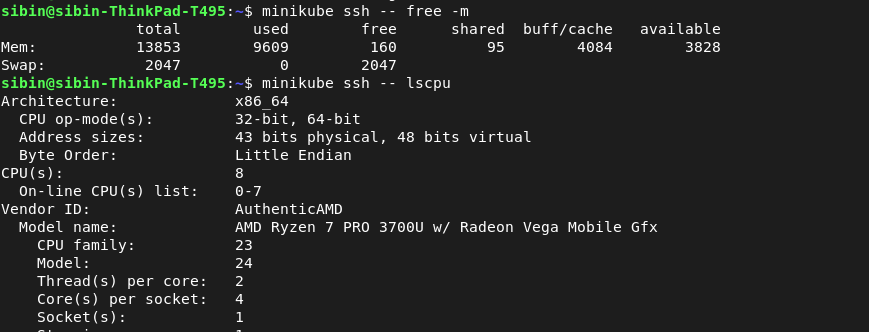
\includegraphics[width=0.8\textwidth]{implementation/minikube-cpunmem.png}
    \caption{Minikube CPU and Memory Usage}
    \label{fig:minikube-cpu-and-memory}
\end{figure}

Since Minikube operates within a container, it leverages the host operating system's kernel and configuration by default. This setup allows the Kubernetes cluster to access additional resources from the host, optimizing performance and scalability for local development and testing.

% Describing kubectl installation
It is important to note that \texttt{kubectl}, the Kubernetes command-line tool, is automatically installed alongside Minikube. To confirm the pods are running in the cluster, run the following command:

\begin{lstlisting}[breaklines=true,basicstyle=\small\ttfamily,frame=single]
kubectl get pods
\end{lstlisting}

% Including figure for kubectl presence
\begin{figure}[h!]
    \centering
    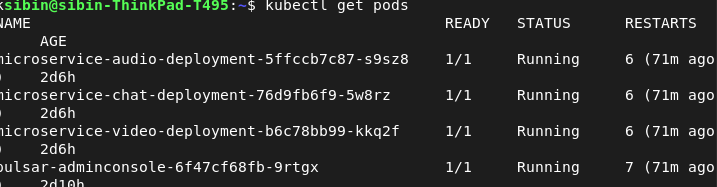
\includegraphics[width=0.8\textwidth]{implementation/pods.png}
    \caption{Verification of Kubectl Presence}
    \label{fig:kgetpods}
\end{figure}

% Confirming successful installation
The Minikube cluster and Kubernetes have been successfully installed and configured on the system. This setup provides a fully working local Kubernetes setup which is ready for deploying and managing applications.

% \section{Installation of Minikube}
% Firstly the host os of the machine at work is Linux Mint which is debian based operating system. An installation for this specific platform is needed. 


% curl -LO https://github.com/kubernetes/minikube/releases/latest/download/minikube-linux-amd64
% sudo install minikube-linux-amd64 /usr/local/bin/minikube && rm minikube-linux-amd64
% Now minikube is successfully installed and working which is verified by

% minikube start

% Note that minikube start starts to run with docker interface by default. It runs on a docker container providing logical seperation.

% \begin{figure}[h!]
% \centering
% 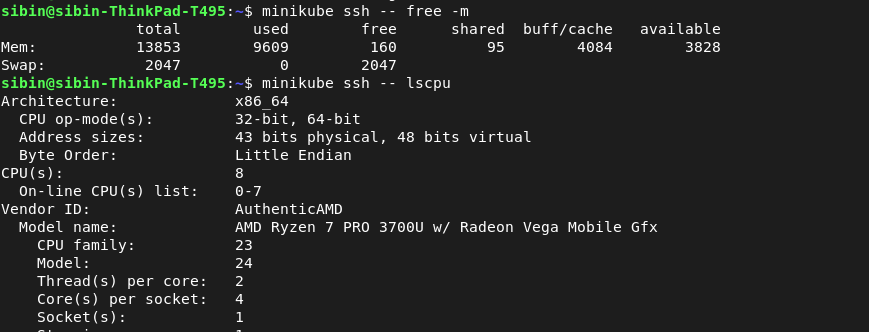
\includegraphics[width=0.8\textwidth]{implementation/minikube-cpunmem.png}
% \caption{Minikube CPU and Memory}
% \label{fig:minikube-cpu-and-memory}
% \end{figure}
% Note that since we run it in a container, it uses host operating system's operating system and configuration by default. This allows us to use more resources for our kubernetes cluster.

% It is to note that kubectl is installed by default when minikube is installed. We can check the existance of pods by running kubectl get pods

% \begin{figure}[h!]
% \centering
% 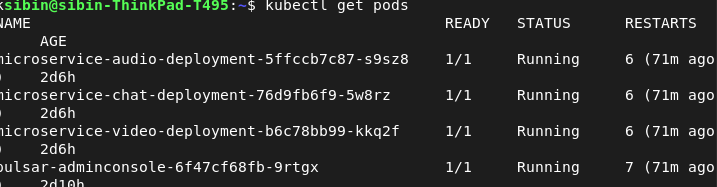
\includegraphics[width=0.8\textwidth]{implementation/pods.png}
% \caption{Kubectl Presence}
% \label{fig:kgetpods}
% \end{figure}

% The minikube cluster and kubernetes have been successfully installed in the system.

% \section{Configuration Metal-lb}
% Metal-lb is a loadbalancer which operates at Layer 4 which is required for exposing all services of type load balancer in our kubernetes cluster. Minikube provides with easy installation with addons options

% minikube addons list
% It lists several addons provided by minikube. In it it can be seen that metallb is disabled which needs to be enabled so to enable it run the following command

% minikube addons enable metal-lb

% Now the metallb requires a range of ip addresses so it can assign to services created within kubernetes

% When minikube container was started with minikube start, it created a network interface in background for minikube ie kubernetes environment which can be verifed with 
% ifconfig. For machine at use, it the interface was name was br-5d.. and had values  inet 192.168.49.1  netmask 255.255.255.0  broadcast 192.168.49.255. This essentially meant the last octet is open from 0-255, which creates a subnet and can be represented by
% 192.168.49.0/24. 
% minikube addons configure metallb
% Enter Load Balancer Start IP: 192.168.49.1
% Enter Load Balancer End IP: 192.168.49.250
% This configures load balancer for these ip address ranges




% Describing MetalLB configuration process
\section{Configuration of MetalLB}
MetalLB is a load balancer that operates at Layer 4, which is essential for exposing all services of type LoadBalancer in our Kubernetes cluster. Minikube provides a straightforward installation process for MetalLB through its addons feature.

% Listing available addons
To see the existing addons in Minikube, run the following command:

\begin{lstlisting}[breaklines=true,basicstyle=\small\ttfamily,frame=single]
minikube addons list
\end{lstlisting}

This command lists several addons provided by Minikube. Among them, you will notice that MetalLB is disabled by default. To enable it, the following command is executed:

\begin{lstlisting}[breaklines=true,basicstyle=\small\ttfamily,frame=single]
minikube addons enable metallb
\end{lstlisting}

% Explaining IP range configuration for MetalLB
MetalLB requires a range of IP addresses to assign to services created within the Kubernetes cluster. When the Minikube container was started with the \texttt{minikube start} command, it created a network interface in the background for the Minikube (i.e., Kubernetes) environment. This can be verified by running:

\begin{lstlisting}[breaklines=true,basicstyle=\small\ttfamily,frame=single]
ifconfig
\end{lstlisting}

For the machine in use, the network interface was named \texttt{br-5d..} and had the following values: \texttt{inet 192.168.49.1}, \texttt{netmask 255.255.255.0}, \texttt{broadcast 192.168.49.255}. This indicates that the last octet is open from 0 to 255 which creates a subnet that can be represented by \texttt{192.168.49.0/24}.

% Configuring MetalLB IP range
To configure MetalLB with appropriate IP address ranges, run the following command:

\begin{lstlisting}[breaklines=true,basicstyle=\small\ttfamily,frame=single]
minikube addons configure metallb
\end{lstlisting}

During configuration, it would prompt asking to enter the start and end IP addresses for the load balancer:

\begin{lstlisting}[breaklines=true,basicstyle=\small\ttfamily,frame=single]
Enter Load Balancer Start IP: 192.168.49.1
Enter Load Balancer End IP: 192.168.49.250
\end{lstlisting}

This configures the MetalLB load balancer to expose applications within the specified IP address range, enabling it to assign IPs to LoadBalancer-type services in the Kubernetes cluster.

% \section{Wireshark}
% To install wireshark and successfully capture traffic, the following process was followed.
% sudo apt install wireshark
% wireshark 
% this opens out wireshark
% It asks you to monitor a specific network interface which when selected started capturing realtime traffic to and from the network interface. Here its to note that higher level application protocols which are encrypted can be captured but not looked into due to their encryption with standard tls protocol. We need tls session keys which would help us decrypt the communication. The session keys can either be logged from the client and server and can be loaded from
% edit->preferences->protcols->tls->premaster secret log name->load the tls session keys

% This process helps to decrypt the TLS encrypted data captured over the network.


% Describing Wireshark installation and usage process
\section{Network Traffic Capture}
To install Wireshark and successfully capture network traffic on Linux Mint OS, the following process was followed.

% Providing installation commands
\subsection{Run Commands}
First, install Wireshark using the package manager by executing the following command:

\begin{lstlisting}[breaklines=true,basicstyle=\small\ttfamily,frame=single]
sudo apt install wireshark
\end{lstlisting}

Launch Wireshark by running:

\begin{lstlisting}[breaklines=true,basicstyle=\small\ttfamily,frame=single]
wireshark
\end{lstlisting}

Above command opens up the Wireshark application. Upon launching, Wireshark prompts you to select a specific network interface to monitor. Once an interface is selected, Wireshark begins capturing real-time traffic to and from the chosen network interface.



% Describing Chromium TLS key logging process
\subsection{Logging Chromium Client TLS Keys}
To log the TLS session keys for the Chromium client, the following steps were performed to ensure proper configuration and logging of the keys for use in decrypting network traffic.

% Providing commands for logging TLS keys
First, terminate any running instances of Chromium by executing the following command:

\begin{lstlisting}[breaklines=true,basicstyle=\small\ttfamily,frame=single]
pkill chromium
\end{lstlisting}

Next, set the environment variable to specify the path for the TLS key log file:

\begin{lstlisting}[breaklines=true,basicstyle=\small\ttfamily,frame=single]
export SSLKEYLOGFILE=$HOME/premaster-secret/sslkeylogfile.log
\end{lstlisting}

Then, restart Chromium to begin logging the TLS keys to the specified path.

% Including figure for SSL key log
\begin{figure}[h!]
    \centering
    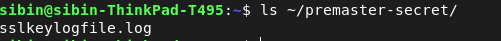
\includegraphics[width=0.8\textwidth]{implementation/sslkeylog.png}
    \caption{Chromium Client's SSL Key Log}
    \label{fig:chromiumssl}
\end{figure}

\subsection{Configuring TLS Keys in Wireshark}

This process successfully logs the TLS session keys to the designated file, enabling the decryption of TLS-encrypted traffic captured from the Chromium client.

% Explaining limitations and TLS decryption
It is important to note that higher-level application protocols, which are encrypted using the standard TLS protocol, can be captured but cannot be inspected directly due to their encryption. To decrypt such communications, TLS session keys are required. These session keys can be logged from the client or server and loaded into Wireshark for decryption.

% Configuring Wireshark for TLS decryption
To decrypt TLS traffic, TLS session keys must be loaded and to load the keys, following steps in Wireshark were followed:

\begin{enumerate}
    \item Go to \texttt{Edit -> Preferences -> Protocols -> TLS}.
    \item In the TLS settings, locate the \texttt{Pre-Master Secret Log Filename} field.
    \item Load the TLS session keys by adding the path of the log file which contain the keys.
\end{enumerate}

This process enables Wireshark to decrypt the TLS-encrypted data captured over the network, allowing for detailed inspection of the communication.



% \subsection{Logging Chromium Client TLS keys}
% killing running instance of chromium -> pkill chromium
% export SSLKEYLOGFILE=$HOME/premaster-secret/sslkeylogfile.log
% and starting the chromium again
% This logs the keys to the specified path
% \begin{figure}[h!]
% \centering
% 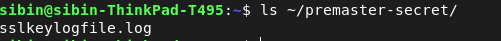
\includegraphics[width=0.8\textwidth]{implementation/sslkeylog.png}
% \caption{Chromium Client's SSLKEYLOG}
% \label{fig:chromiumssl}
% \end{figure}


% \section{Certificate Management Process}
% The first step to working with the state of the art Webtransport Streams Http3 Router, it was identified that a need for certificate is substantial as without which the data could not be sent over the specified protocol. Since it was not feasible to own a domain as approach to creating a self signed certificate was taken.

% The following commands created a self signed certificate for a new domain

% openssl req -x509 -newkey rsa:4096 -keyout tls.key -out tls.crt -days 365 -nodes -subj "/CN=quic-aioquic.com:

% This requests openssl for a rsa keypair and creates cert and key with an expiry of 365 days with the Subject alternative name and CName set to the custo domain quic-aioquic.com
% Now in order to use the certificate the client must forward request to the particular domain and the client must itself trust the domain. In order to do that and snce we were working with browser client chrome. Through settings we could upload the certificate

% Settings -> Privary and Security -> Manage Certificates -> Installed Certificates by You -> Import

% This way the client can be trusted





% Describing certificate management process
\section{Certificate Management}
To enable secure communication with the state-of-the-art WebTransport Streams HTTP/3 Router, it was determined that a certificate is essential, as data transmission over the specified protocol requires encryption. Since acquiring a domain was not feasible, the approach of creating a self-signed certificate was adopted.

% Providing commands for creating a self-signed certificate
The following command was used to generate a self-signed certificate for a custom domain:

\begin{lstlisting}[breaklines=true,basicstyle=\small\ttfamily,frame=single]
openssl req -x509 -newkey rsa:4096 -keyout tls.key -out tls.crt -days 365 -nodes -subj "/CN=quic-aioquic.com"
\end{lstlisting}

This command instructs OpenSSL to create an RSA key pair, generating both a certificate (\texttt{tls.crt}) and a private key (\texttt{tls.key}) with an expiration period of 365 days. The \texttt{-nodes} flag ensures the private key is not encrypted, and the Subject Alternative Name and Common Name (CN) are set to the custom domain \texttt{quic-aioquic.com}.

% Explaining certificate usage and client configuration
To utilize the certificate, the client must forward requests to the specified domain, and the client itself must trust the domain. Since the client in use was the Chrome browser, the self-signed certificate was imported through the browser's settings to establish trust.

% Providing steps for importing the certificate in Chrome
The certificate can be imported by following these steps in Chrome:

\begin{enumerate}
    \item Navigate to \texttt{Settings -> Privacy and Security -> Manage Certificates}.
    \item Under the \texttt{Installed Certificates by You} section, select \texttt{Import}.
    \item Follow the prompts to upload the \texttt{tls.crt} certificate file.
\end{enumerate}

This process ensures that the Chrome client trusts the self-signed certificate, enabling secure communication with the WebTransport Streams HTTP/3 Router.


% \section{DNS entry}
% In order to work with a DNS entry for your local setup we need a domain name resolution process to be in place. Now that the certificates are structed, requests are explictly checked for the domain. For the linux machine, the configuration changes was done to /etc/hosts directory where an entry for dns was inputted. for my system I added this line

% 192.168.49.201 quic-aioquic.com
% It maps the domain name to the specific ip address


% Describing DNS entry configuration process
\section{DNS Entry Configuration}
To enable domain name resolution for the local setup, a DNS entry must be configured. With the certificates properly structured, requests are explicitly checked for the specified domain. On a Linux machine, this configuration is achieved by modifying the \texttt{/etc/hosts} file to include a DNS entry that maps the domain to a specific IP address.

% Providing the DNS entry configuration
For the system in use, the following line was added to the \texttt{/etc/hosts} file:

\begin{lstlisting}[breaklines=true,basicstyle=\small\ttfamily,frame=single]
192.168.49.201 quic-aioquic.com
\end{lstlisting}

This entry maps the domain name \texttt{quic-aioquic.com} to the IP address \texttt{192.168.49.201}, ensuring proper domain name resolution for the local setup.




% Describing the client construction process
\section{Client Construction}
The construction of the client was accomplished using several core components, each designed to ensure a robust and user-friendly streaming experience. These components are detailed below.

% Describing the user interface design
\subsection{User Interface Design}
The client's user interface is created for clarity and functionality, offering an intuitive overview of the streaming process. The layout is structured using a responsive \textbf{CSS Grid} (\texttt{.container}), which divides the main content into distinct panels for streamlined user interaction.

\begin{itemize}
    \item \textbf{Video \& Audio Stream Panel} (\texttt{.panel}): This panel prominently displays the local video feed (\texttt{<video id="localVideo">}) and includes controls for initiating or stopping streaming, toggling video quality, and starting or stopping optional file and screen data streams.
    \item \textbf{Live Chat Panel} (\texttt{.panel}): This features a scrollable message display area (\texttt{.chat-\allowbreak{}messages}) and an input field with a send button (\texttt{.chat-input}) for real-time text communication.
    \item \textbf{Metrics Display} (\texttt{.metrics}): This provides at-a-glance performance indicators, including the count of video frames, audio packets, chat messages sent, and the calculated data transfer rate.
    \item \textbf{Status Bar} (\texttt{\#status}): This offers immediate feedback on the WebTransport connection state.
    \item \textbf{System Logs Panel} (\texttt{.logs}): This acts as a console, displaying critical information about stream creation, packet transmission, and error events, which is essential for monitoring and debugging during development and testing.
\end{itemize}

The visual design adopts a dark theme using CSS, enhancing readability in low-light conditions and providing a modern aesthetic. Buttons are styled with distinct colors (\texttt{.btn-start}, \texttt{.btn-stop}, \texttt{.btn-toggle}) to clearly indicate their actions and current states, such as \texttt{disabled} styling.

% Describing WebTransport connection setup
\subsection{WebTransport Connection Setup}
Establishing a reliable connection to the WebTransport server is the foundational step for all streaming operations. This is managed within the \texttt{WebTransportStreamer} class's \texttt{startStreaming()} method. The connection is initiated by creating a new \texttt{WebTransport} instance, specifying the server URL (\texttt{https://quic-aioquic.com:4433/wt}), which points to the secure QUIC endpoint of the server.

\begin{lstlisting}[breaklines=true,basicstyle=\small\ttfamily,frame=single]
//Initialize WebTransport connection to the server endpoint
this.transport = new WebTransport(this.serverUrl);
\end{lstlisting}

To ensure robust operation, event listeners are set up for \textbf{connection state changes} (\texttt{this.transport.onstatechange}) and \textbf{errors} (\texttt{this.transport.onerror}). These listeners are critical for monitoring the connection's health:

\begin{itemize}
    \item \texttt{onstatechange}: Updates the UI status and triggers \texttt{stopStreaming()} if the connection \texttt{state} transitions to \texttt{'closed'}, indicating a graceful shutdown or an unexpected termination.
    \item \texttt{onerror}: Catches any underlying transport errors, logs them to the console, and initiates \texttt{stopStreaming()} to clean up resources.
\end{itemize}

\begin{lstlisting}[breaklines=true,basicstyle=\small\ttfamily,frame=single]
this.transport.onstatechange = () => {
    this.log(`Transport state: ${this.transport.state}`, 'info');
    if (this.transport.state === 'closed') {
        this.stopStreaming();
    }
};
this.transport.onerror = (event) => {
    this.log(`Transport error: ${event.message}`, 'error'); #logs error
    this.stopStreaming();
};
\end{lstlisting}

The \texttt{await this.transport.ready;} promise ensures that the application waits until the WebTransport connection is established before starting with media capture and stream creation which prevents operations on a disconnected transport. This ensures a stable foundation for subsequent streaming activities.

% Describing media capture and stream initialization
\subsection{Media Capture and Stream Initialization}
Once the WebTransport connection is ready, the client proceeds to capture local media and prepare the data streams for transmission.

\subsubsection{Video/Audio Capture}
Media access is prompted using the \textbf{WebRTC \texttt{getUserMedia} API}, this requests the user for permission to access camera and microphone. The \texttt{constraints} object defines the desired media properties:

\begin{itemize}
    \item \texttt{video}: Configured for resolutions \texttt{640x480} at \texttt{15fps} (Standard Quality) or \texttt{1280x720} at \texttt{30fps} (High Quality), with change of the \texttt{isHighQuality} flag.
    \item \texttt{audio}: Includes \texttt{echoCancellation} and \texttt{noiseSuppression} to improve audio clarity.
\end{itemize}

\begin{lstlisting}[breaklines=true,basicstyle=\small\ttfamily,frame=single]
const mediaConstraints = {
    video: {
        //Set video dimensions based on quality mode selection
        width: this.isHighQuality ? 1280 : 640,
        height: this.isHighQuality ? 720 : 480,
        //Configure frame rate for optimal performance
        frameRate: this.isHighQuality ? 30 : 15
    },
    audio: {
        //Apply audio processing enhancements
        echoCancellation: true,
        noiseSuppression: true
    }
};
//Capture user media with specified constraints
this.mediaStream = await navigator.mediaDevices.getUserMedia(mediaConstraints);
//Display captured video in local preview element
this.elements.localVideo.srcObject = this.mediaStream;
\end{lstlisting}

The captured \texttt{mediaStream} is assigned to the \texttt{<video id="localVideo">} element, allowing the user to see their own video feed. A \texttt{Promise} is used to wait for the video element to trigger \texttt{loadeddata}, ensuring the media stream is fully ready before processing.

\subsubsection{Stream Creation}
WebTransport's strength lies in its support for \textbf{multiplexing} via individual streams over a single connection. The client leverages \textbf{unidirectional streams} (\texttt{create\allowbreak{}Bidirectional\allowbreak{}Stream()}) for each distinct data type:

\begin{itemize}
    \item \texttt{this.videoStream}: For outgoing video frames.
    \item \texttt{this.audioStream}: For outgoing audio packets.
    \item \texttt{this.chatStream}: For outgoing chat messages.
    \item \texttt{this.fileStream}: For sending arbitrary file data.
    \item \texttt{this.screenStream}: For sending screen share data.
\end{itemize}

\begin{lstlisting}[breaklines=true,basicstyle=\small\ttfamily,frame=single]
#Initialize separate WebTransport streams for different data types
#Video stream for transmitting video frame data
this.videoStream = await this.transport.createUnidirectionalStream();
#Audio stream for transmitting audio packet data  
this.audioStream = await this.transport.createUnidirectionalStream();
#Chat stream for transmitting text messages
this.chatStream = await this.transport.createUnidirectionalStream();
\end{lstlisting}

With separate unidirectional streams, the client sends different types of data independently without head-of-line blocking, enhancing real-time performance and simplifying server-side processing.

% Describing packet construction and sending
\subsection{Packet Construction and Sending}
A custom packet format is implemented to encapsulate various data types for transmission over WebTransport streams, allowing the server to easily identify and process incoming data.

\subsubsection{Packet Format}
Each packet that is sent over a WebTransport stream follows a predefined format consisting of a \textbf{32-byte header} followed by a variable-length \textbf{payload}. The header provides essential metadata:

\begin{itemize}
    \item \textbf{\texttt{track\_id} (16 bytes)}: A string identifier, such as \texttt{'live\_video'}, \texttt{'test\_audio'}, \texttt{'live\_chat'}, used by the receiver to identify the packet's content within its stream and is padded with null bytes if it's shorter than 16 bytes.
    \item \textbf{\texttt{payload\_length} (4 bytes)}: A 32-bit unsigned integer that indicates the exact size of the payload in bytes which is required for correct payload reading.
    \item \textbf{\texttt{track\_type} (12 bytes)}: A string, such as \texttt{'video'}, \texttt{'audio'}, \texttt{'chat'}, \texttt{'file'}, \texttt{'screen'}, classifying the general type of data, padded to 12 bytes.
\end{itemize}

The \texttt{buildPacket()} function assembles this structure:

\begin{lstlisting}[breaklines=true,basicstyle=\small\ttfamily,frame=single]
buildPacket(trackId, trackType, payload, forceSize = null) {
    let finalPayload = payload;
    if (forceSize && forceSize > payload.length) {
        finalPayload = new Uint8Array(forceSize);
        finalPayload.set(payload, 0);
        for (let i = payload.length; i < forceSize; i++) { #Padding
            finalPayload[i] = i % 256; //Padding pattern
        }
    }

    const header = new ArrayBuffer(32);
    const view = new DataView(header);
    //Set track_id (bytes 0-15)
    new Uint8Array(header, 0, 16).set(this.encoder.encode(trackId.substring(0, 16)));
    //Set payload_length (bytes 16-19)
    view.setUint32(16, finalPayload.length, false); //false for big-endian
    //Set track_type (bytes 20-31)
    new Uint8Array(header, 20, 12).set(this.encoder.encode(trackType.substring(0, 12)));

    const packet = new Uint8Array(header.byteLength + finalPayload.length);
    packet.set(new Uint8Array(header), 0);
    packet.set(finalPayload, header.byteLength);
    this.bytesTransferred += packet.length;
    return packet;
}
\end{lstlisting}

The \texttt{forceSize} parameter allows the client to artificially inflate packet size with padding, serving as a testing feature to analyze the impact of larger packets on network performance and server-side buffer management.

\subsubsection{Sending Logic}
Data is sent using the \texttt{WritableStreamDefaultWriter} associated with each WebTransport stream. The \texttt{loggedWrite()} helper function wraps the \texttt{writer.write()} operation, providing robust error handling and immediate logging feedback:

\begin{lstlisting}[breaklines=true,basicstyle=\small\ttfamily,frame=single]
//Asynchronous function to send packets with comprehensive error handling
async transmitWithLogging(streamWriter, packetData, dataType) {
    try {
        //Attempt to write packet data to the WebTransport stream
        await streamWriter.write(packetData);
        //Log successful transmission with packet details
        this.log(`Successfully transmitted ${dataType} packet: ${packetData.length} bytes`, 'success');
        return true;
    } catch (transmissionError) {
        //Log detailed error information for debugging
        this.log(`Transmission failed for ${dataType} packet: ${transmissionError.message}`, 'error');
        return false;
    }
}
\end{lstlisting>

This function logs every successful packet transmission, including its type and size, aiding in real-time monitoring. In case of failure, such as stream closed, network issue, an error is logged, ensuring communication issues are immediately visible. The \texttt{writer.releaseLock()} is used after sending test packets to allow re-acquisition for continuous streaming.

% Describing video streaming implementation
\subsection{Video Streaming Implementation}
Video streaming is handled by continuously capturing frames from the local video feed, processing them, and sending them over the dedicated video WebTransport stream. The \texttt{startVideoCapture()} method uses a hidden \texttt{HTMLCanvasElement} as an intermediary to process video frames:

\begin{lstlisting}[breaklines=true,basicstyle=\small\ttfamily,frame=single]
const canvas = document.createElement('canvas');
const ctx = canvas.getContext('2d');
canvas.width = this.isHighQuality ? 1280 : 640;
canvas.height = this.isHighQuality ? 720 : 480;
this.videoWriter = this.videoStream.getWriter();
\end{lstlisting}

A \texttt{captureLoop()} function recursively calls itself using \texttt{setTimeout} to maintain a consistent frame rate (15 FPS for standard quality, 30 FPS for high quality). The loop includes:

\begin{enumerate}
    \item \textbf{Frame Capture}: \texttt{ctx.drawImage(this.elements.localVideo, 0, 0, canvas.width\allowbreak{}, canvas.height);} draws the current video frame onto the canvas.
    \item \textbf{Encoding}: \texttt{canvas.toDataURL('image/jpeg', quality);} converts the canvas content into a JPEG image data URL, with \texttt{quality} set to 0.7 for standard or 0.9 for high quality.
    \item \textbf{Binary Conversion}: The Base64-encoded image data is converted into a \texttt{Uint8Array} payload.
    \item \textbf{Packetization and Sending}: The \texttt{buildPacket()} method creates a packet with \texttt{track\_id 'live\_video'} and \texttt{track\_type 'video'}, applying a \texttt{forceSize} of 2500 bytes for high-quality streaming to test network handling. The packet is sent via \texttt{this.loggedWrite(this.videoWriter, packet, 'VIDEO')}.
    \item \textbf{Metrics Update}: \texttt{this.videoFrameCount++} increments the counter for UI display.
\end{enumerate}

This approach provides granular control over video encoding and packet size, facilitating experimental analysis of quality settings and packet sizes.

% Describing audio streaming implementation
\subsection{Audio Streaming Implementation}
Audio streaming leverages the \textbf{Web Audio API} for efficient capture and processing of microphone input. The \texttt{startAudioCapture()} method sets up an audio processing pipeline:

\begin{lstlisting}[breaklines=true,basicstyle=\small\ttfamily,frame=single]
const audioContext = new (window.AudioContext || window.webkitAudioContext)();
await audioContext.resume();
const source = audioContext.createMediaStreamSource(this.mediaStream);
const processor = audioContext.createScriptProcessor(4096, 1, 1);
this.audioWriter = this.audioStream.getWriter();
\end{lstlisting}

\begin{itemize}
    \item \textbf{\texttt{AudioContext}}: Provides the framework for audio processing, with \texttt{audioContext.re\allowbreak{}sume()} ensuring processing starts.
    \item \textbf{\texttt{MediaStreamSource}}: Creates an audio node from the \texttt{mediaStream} obtained via \texttt{getUserMedia}.
    \item \textbf{\texttt{ScriptProcessorNode}}: Uses a buffer size of 4096 samples with one input and output channel for mono audio.
\end{itemize}

In the \texttt{processor.onaudioprocess} event handler:

\begin{enumerate}
    \item \textbf{Audio Data Extraction}: \texttt{event.inputBuffer.getChannelData(0)} retrieves raw floating-point audio samples.
    \item \textbf{PCM Conversion}: Samples are converted to 16-bit PCM format:
    \begin{lstlisting}[breaklines=true,basicstyle=\small\ttfamily,frame=single]
const pcmData = new Int16Array(inputData.length);
for (let i = 0; i < inputData.length; i++) {
    pcmData[i] = Math.max(-32768, Math.min(32767, inputData[i] * 32768));
}
const payload = new Uint8Array(pcmData.buffer);
    \end{lstlisting}
    \item \textbf{Packetization and Sending}: The \texttt{pcmData} is used as the payload for a packet with \texttt{track\_id 'live\_audio'} and \texttt{track\_type 'audio'}, with a \texttt{forceSize} of 2200 bytes for testing. The packet is sent via \texttt{this.loggedWrite(this.audioWriter, packet, 'AUDIO')}.
    \item \textbf{Metrics Update}: \texttt{this.audioPacketCount++} increments the counter.
\end{enumerate}

The \texttt{source} and \texttt{processor} nodes are connected to the \texttt{audioContext.destination}, ensuring an active audio processing chain.

% Describing chat messaging implementation
\subsection{Chat Messaging Implementation}
The live chat functionality enables real-time text communication using a dedicated WebTransport stream. The \texttt{sendChatMessage()} method is triggered when the user presses "Enter" or clicks the "Send" button:

\begin{enumerate}
    \item \textbf{Message Retrieval and Validation}: The message is retrieved from \texttt{this.elements\allowbreak{}.chatInput.value} and trimmed, exiting if empty.
    \item \textbf{Data Structuring}: The message is encapsulated in a JSON object:
    \begin{lstlisting}[breaklines=true,basicstyle=\small\ttfamily,frame=single]
const chatData = {
    message_id: Date.now(),
    timestamp: Date.now(),
    user: 'streamer',
    message: message,
    type: 'text'
};
const payload = this.encoder.encode(JSON.stringify(chatData));
    \end{lstlisting}
    \item \textbf{Packetization and Sending}: The JSON object is encoded into a \texttt{Uint8Array} and passed to \texttt{buildPacket()} with \texttt{track\_id 'live\_chat'} and \texttt{track\_type 'chat'}, then sent via \texttt{this.loggedWrite()}.
    \item \textbf{Local Display and Metrics}: The message is appended to \texttt{this.elements.chatMe\allowbreak{}ssages}, scrolled to the bottom, the input field is cleared, and \texttt{this.chatMessageCount++} is incremented.
\end{enumerate}

This dedicated chat stream ensures low-latency communication, critical for interactive applications.


% \section{Client Construction}
% Construction of Client was done with several core components. They are explained below.

% \subsection{User Interface Design}
% The client's user interface is designed for clarity and functionality, providing an intuitive overview of the streaming process. The layout is structured using a responsive \textbf{CSS Grid} (\texttt{.container}), dividing the main content into distinct panels.
% \begin{itemize}
%     \item The \textbf{Video \& Audio Stream panel} (\texttt{.panel}) prominently displays the local video feed (\texttt{<video id="localVideo">}) and contains controls for initiating/stopping streaming, toggling video quality, and starting/stopping the optional file and screen data streams.
%     \item The \textbf{Live Chat panel} (\texttt{.panel}) features a scrollable message display area (\texttt{.chat-messages}) and an input field with a send button (\texttt{.chat-input}) for real-time text communication.
%     \item A dedicated \textbf{Metrics display} (\texttt{.metrics}) provides at-a-glance performance indicators, including the count of video frames, audio packets, chat messages sent, and the calculated data transfer rate.
%     \item A \textbf{Status bar} (\texttt{\#status}) offers immediate feedback on the WebTransport connection state.
%     \item Finally, the \textbf{System Logs panel} (\texttt{.logs}) acts as a console, displaying crucial information about stream creation, packet transmission, and error events, vital for monitoring and debugging during development and testing.
% \end{itemize}
% The visual design adopts a dark theme using CSS, enhancing readability in low-light conditions and providing a modern aesthetic. Buttons are styled with distinct colors (\texttt{.btn-start}, \texttt{.btn-stop}, \texttt{.btn-toggle}) to clearly indicate their actions and current states (e.g., \texttt{disabled} styling).

% \subsection{WebTransport Connection Setup}
% Establishing a reliable connection to the WebTransport server is the foundational step for all streaming operations. This is managed within the \texttt{WebTransportStreamer} class's \texttt{startStreaming()} method.
% The connection is initiated by creating a new \texttt{WebTransport} instance, specifying the server URL (\texttt{this.serverUrl = 'https://quic-aioquic.com:4433/wt'}). This URL points to the secure QUIC endpoint of the server.
% \begin{verbatim}
% this.transport = new WebTransport(this.serverUrl);
% \end{verbatim}
% To ensure robust operation, event listeners are set up for \textbf{connection state changes} (\texttt{this.transport.onstatechange}) and \textbf{errors} (\texttt{this.transport.onerror}). These listeners are critical for monitoring the connection's health:
% \begin{itemize}
%     \item \texttt{onstatechange}: Updates the UI status and triggers \texttt{stopStreaming()} if the connection \texttt{state} transitions to \texttt{'closed'}, indicating a graceful shutdown or an unexpected termination.
%     \item \texttt{onerror}: Catches any underlying transport errors, logs them to the console, and also initiates \texttt{stopStreaming()} to clean up resources.
% \end{itemize}
% \begin{verbatim}
% this.transport.onstatechange = () => {
%     this.log(`Transport state: ${this.transport.state}`, 'info');
%     if (this.transport.state === 'closed') {
%         this.stopStreaming();
%     }
% };
% this.transport.onerror = (event) => {
%     this.log(`Transport error: ${event.message}`, 'error');
%     this.stopStreaming();
% };
% \end{verbatim}
% The \texttt{await this.transport.ready;} promise ensures that the application waits until the WebTransport connection is fully established before proceeding with media capture and stream creation, preventing operations on a disconnected transport. This ensures a stable foundation for subsequent streaming activities.

% \subsection{Media Capture and Stream Initialization}
% Once the WebTransport connection is ready, the client proceeds to capture local media and prepare the data streams for transmission.

% \subsubsection{Video/Audio Capture}
% Media access is requested using the \textbf{WebRTC \texttt{getUserMedia} API}. This API prompts the user for permission to access their camera and microphone. The \texttt{constraints} object defines the desired media properties:
% \begin{itemize}
%     \item \texttt{video}: Configured for either \texttt{640x480} at \texttt{15fps} (Standard Quality) or \texttt{1280x720} at \texttt{30fps} (High Quality), controlled by the \texttt{isHighQuality} flag.
%     \item \texttt{audio}: Includes \texttt{echoCancellation} and \texttt{noiseSuppression} to improve audio clarity.
% \end{itemize}
% \begin{verbatim}
% const constraints = {
%     video: {
%         width: this.isHighQuality ? 1280 : 640,
%         height: this.isHighQuality ? 720 : 480,
%         frameRate: this.isHighQuality ? 30 : 15
%     },
%     audio: {
%         echoCancellation: true,
%         noiseSuppression: true
%     }
% };
% this.mediaStream = await navigator.mediaDevices.getUserMedia(constraints);
% this.elements.localVideo.srcObject = this.mediaStream;
% \end{verbatim}
% The captured \texttt{mediaStream} is then assigned to the \texttt{<video id="localVideo">} element, allowing the user to see their own video feed. A \texttt{Promise} is used to wait for the video element to \texttt{loadeddata}, ensuring the media stream is fully ready before attempting to process it.

% \subsubsection{Stream Creation}
% WebTransport's core strength for streaming lies in its support for \textbf{multiplexing} via individual streams over a single connection. The client leverages \textbf{unidirectional streams} (\texttt{createUnidirectionalStream()}) for each distinct data type:
% \begin{itemize}
%     \item \texttt{this.videoStream}: For outgoing video frames.
%     \item \texttt{this.audioStream}: For outgoing audio packets.
%     \item \texttt{this.chatStream}: For outgoing chat messages.
%     \item \texttt{this.fileStream}: For sending arbitrary file data.
%     \item \texttt{this.screenStream}: For sending screen share data.
% \end{itemize}

% \begin{verbatim}
% this.videoStream = await this.transport.createUnidirectionalStream();
% this.audioStream = await this.transport.createUnidirectionalStream();
% this.chatStream = await this.transport.createUnidirectionalStream();
% \end{verbatim}

% By using separate unidirectional streams, the client can send different types of data independently without head-of-line blocking, enhancing real-time performance and simplifying server-side processing, as each stream carries a dedicated data type.

% \subsection{Packet Construction and Sending}
% A custom packet format is implemented to encapsulate various data types for transmission over WebTransport streams. This structured approach allows the server to easily identify and process incoming data.

% \subsubsection{Packet Format}
% Each packet sent over a WebTransport stream adheres to a predefined format consisting of a \textbf{32-byte header} followed by a variable-length \textbf{payload}. The header provides essential metadata:
% \begin{itemize}
%     \item \textbf{\texttt{track\_id} (16 bytes):} A string identifier (e.g., \texttt{'live\_video'}, \texttt{'test\_audio'}, \texttt{'live\_chat'}) used by the receiver to identify the content of the packet within its stream. It's padded with null bytes if shorter than 16 bytes.
%     \item \textbf{\texttt{payload\_length} (4 bytes):} A 32-bit unsigned integer (big-endian) indicating the exact size of the payload in bytes. This is crucial for the receiver to correctly read the payload.
%     \item \textbf{\texttt{track\_type} (12 bytes):} A string (e.g., \texttt{'video'}, \texttt{'audio'}, \texttt{'chat'}, \texttt{'file'}, \texttt{'screen'}) classifying the general type of data carried by the packet. Similar to \texttt{track\_id}, it's padded to 12 bytes.
% \end{itemize}

% The \texttt{buildPacket()} function is responsible for assembling this structure:
% \begin{verbatim}
% buildPacket(trackId, trackType, payload, forceSize = null) {
%     let finalPayload = payload;
%     if (forceSize && forceSize > payload.length) {
%         finalPayload = new Uint8Array(forceSize);
%         finalPayload.set(payload, 0);
%         for (let i = payload.length; i < forceSize; i++) {
%             finalPayload[i] = i % 256; // Padding pattern
%         }
%     }

%     const header = new ArrayBuffer(32);
%     const view = new DataView(header);
%     // Set track_id (bytes 0-15)
%     new Uint8Array(header, 0, 16).set(this.encoder.encode(trackId.substring(0, 16)));
%     // Set payload_length (bytes 16-19)
%     view.setUint32(16, finalPayload.length, false); // false for big-endian
%     // Set track_type (bytes 20-31)
%     new Uint8Array(header, 20, 12).set(this.encoder.encode(trackType.substring(0, 12)));

%     const packet = new Uint8Array(header.byteLength + finalPayload.length);
%     packet.set(new Uint8Array(header), 0);
%     packet.set(finalPayload, header.byteLength);
%     this.bytesTransferred += packet.length;
%     return packet;
% }
% \end{verbatim}
% A notable feature is the \texttt{forceSize} parameter, allowing the client to artificially inflate the packet size with padding. This is a crucial \textbf{testing feature} used to analyze the impact of larger packets on network performance and server-side buffer management.

% \subsubsection{Sending Logic}
% Data is sent using the \texttt{WritableStreamDefaultWriter} associated with each WebTransport stream. The \texttt{loggedWrite()} helper function wraps the \texttt{writer.write()} operation, providing robust error handling and immediate logging feedback.
% \begin{verbatim}
% async loggedWrite(writer, packet, streamType) {
%     try {
%         await writer.write(packet);
%         this.log(`Sent ${streamType} packet: ${packet.length} bytes`, 'success');
%         return true;
%     } catch (error) {
%         this.log(`Failed to send ${streamType} packet: ${error.message}`, 'error');
%         return false;
%     }
% }
% \end{verbatim}
% This function logs every successful packet transmission, including its type and size, aiding in the real-time monitoring of data flow. In case of failure (e.g., stream closed, network issue), an error is logged, ensuring that communication problems are immediately visible. The \texttt{writer.releaseLock()} is used after sending test packets to ensure the writer can be re-acquired for subsequent continuous streaming.

% \subsection{Video Streaming Implementation}
% Video streaming is handled by continuously capturing frames from the local video feed, processing them, and sending them over the dedicated video WebTransport stream.
% The core of video capture occurs within the \texttt{startVideoCapture()} method. A hidden \texttt{HTMLCanvasElement} is used as an intermediary to process video frames:
% \begin{verbatim}
% const canvas = document.createElement('canvas');
% const ctx = canvas.getContext('2d');
% canvas.width = this.isHighQuality ? 1280 : 640;
% canvas.height = this.isHighQuality ? 720 : 480;
% this.videoWriter = this.videoStream.getWriter();
% \end{verbatim}
% A \texttt{captureLoop()} function is defined, which recursively calls itself using \texttt{setTimeout} to maintain a consistent frame rate (15 FPS for standard quality, 30 FPS for high quality). Inside the loop:
% \begin{enumerate}
%     \item \textbf{Frame Capture:} \texttt{ctx.drawImage(this.elements.localVideo, 0, 0, canvas.width, canvas.height);} draws the current video frame onto the canvas.
%     \item \textbf{Encoding:} \texttt{canvas.toDataURL('image/jpeg', quality);} converts the canvas content into a JPEG image data URL. JPEG is chosen for its compression efficiency suitable for video frames. The \texttt{quality} parameter is adjustable (0.7 for standard, 0.9 for high).
%     \item \textbf{Binary Conversion:} The Base64-encoded image data is converted into a \texttt{Uint8Array} payload.
%     \item \textbf{Packetization and Sending:} The \texttt{buildPacket()} method is used to create a packet with \texttt{track\_id 'live\_video'} and \texttt{track\_type 'video'}. For \textbf{high-quality streaming}, a \texttt{forceSize} of \texttt{2500} bytes is applied to test the network's handling of larger video packets. This packet is then sent via \texttt{this.loggedWrite(this.videoWriter, packet, 'VIDEO')}.
%     \item \textbf{Metrics Update:} \texttt{this.videoFrameCount++} increments the counter for display in the UI.
% \end{enumerate}
% This approach provides granular control over video encoding and packet size, allowing for experimental analysis of different quality settings and forced packet sizes over WebTransport.

% \subsection{Audio Streaming Implementation}
% Audio streaming leverages the \textbf{Web Audio API} for efficient capture and processing of microphone input. The \texttt{startAudioCapture()} method sets up an audio processing pipeline:
% \begin{verbatim}
% const audioContext = new (window.AudioContext || window.webkitAudioContext)();
% await audioContext.resume();
% const source = audioContext.createMediaStreamSource(this.mediaStream);
% const processor = audioContext.createScriptProcessor(4096, 1, 1);
% this.audioWriter = this.audioStream.getWriter();
% \end{verbatim}
% \begin{itemize}
%     \item \textbf{\texttt{AudioContext}}: Provides the framework for audio processing. \texttt{audioContext.resume()} is called to ensure audio processing starts even if the browser has initially suspended it.
%     \item \textbf{\texttt{MediaStreamSource}}: \texttt{audioContext.createMediaStreamSource(this.mediaStream)} creates an audio node from the \texttt{mediaStream} obtained from \texttt{getUserMedia}.
%     \item \textbf{\texttt{ScriptProcessorNode}}: \texttt{audioContext.createScriptProcessor(4096, 1, 1)} creates a node that can directly access raw audio data. The first argument (4096) is the buffer size, meaning the \texttt{onaudioprocess} event will fire every time 4096 samples are ready. The second and third arguments specify input and output channel counts (1 for mono).
% \end{itemize}
% Inside the \texttt{processor.onaudioprocess} event handler:
% \begin{enumerate}
%     \item \textbf{Audio Data Extraction:} \texttt{event.inputBuffer.getChannelData(0)} retrieves the raw floating-point audio samples from the first (and only) channel.
%     \item \textbf{PCM Conversion:} The floating-point samples are converted to \textbf{16-bit PCM (Pulse Code Modulation)} format. This is a common uncompressed audio format suitable for streaming.
%     \begin{verbatim}
% const pcmData = new Int16Array(inputData.length);
% for (let i = 0; i < inputData.length; i++) {
%     pcmData[i] = Math.max(-32768, Math.min(32767, inputData[i] * 32768));
% }
% const payload = new Uint8Array(pcmData.buffer);
%     \end{verbatim}
%     \item \textbf{Packetization and Sending:} The \texttt{pcmData} is used as the payload for a packet with \texttt{track\_id 'live\_audio'} and \texttt{track\_type 'audio'}. To test network behavior, a \texttt{forceSize} of \texttt{2200} bytes is applied to audio packets, potentially causing fragmentation or reassembly challenges on the server side. The packet is then sent via \texttt{this.loggedWrite(this.audioWriter, packet, 'AUDIO')}.
%     \item \textbf{Metrics Update:} \texttt{this.audioPacketCount++} increments the counter.
% \end{enumerate}
% The \texttt{source} node is connected to the \texttt{processor}, and the \texttt{processor} is connected to the \texttt{audioContext.destination}, ensuring the audio processing chain is active. This setup provides a continuous stream of raw audio data, allowing for flexible encoding strategies and real-time analysis of audio transmission.

% \subsection{Chat Messaging Implementation}
% The live chat functionality enables real-time text communication between the client and the server. It uses a dedicated WebTransport stream to ensure messages are delivered efficiently and independently of multimedia streams.
% The \texttt{sendChatMessage()} method is triggered when the user presses "Enter" in the chat input or clicks the "Send" button.
% \begin{enumerate}
%     \item \textbf{Message Retrieval and Validation:} The message text is retrieved from \texttt{this.elements.chatInput.value} and trimmed. If empty, the function exits.
%     \item \textbf{Data Structuring:} The message is encapsulated in a JSON object, including a \texttt{message\_id} (current timestamp), \texttt{timestamp}, \texttt{user} (fixed as 'streamer' for this client), the actual \texttt{message} text, and a \texttt{type} ('text'). This structured data simplifies parsing on the server.
%     \begin{verbatim}
% const chatData = {
%     message_id: Date.now(),
%     timestamp: Date.now(),
%     user: 'streamer',
%     message: message,
%     type: 'text'
% };
% const payload = this.encoder.encode(JSON.stringify(chatData));
%     \end{verbatim}
%     \item \textbf{Packetization and Sending:} The JSON object is encoded into a \texttt{Uint8Array} payload using \texttt{TextEncoder} and then passed to \texttt{buildPacket()} with \texttt{track\_id 'live\_chat'} and \texttt{track\_type 'chat'}. This packet is sent over the \texttt{this.chatStream} using \texttt{this.loggedWrite()}.
%     \item \textbf{Local Display and Metrics:} After successful transmission, the message is immediately appended to the local chat display (\texttt{this.elements.chatMessages}), scrolled to the bottom, and the input field is cleared. The \texttt{this.chatMessageCount++} increments the chat message metric.
% \end{enumerate}
% This dedicated chat stream ensures that even under heavy video/audio load, chat messages maintain low latency, critical for interactive communication.


% \subsection{Metrics}
% Robust monitoring is crucial for understanding the client's performance and diagnosing issues, especially in a streaming context. A dedicated \texttt{startMetricsUpdater()} function runs every second via \texttt{setInterval}, updating the UI with key performance indicators:
% \begin{itemize}
%     \item \textbf{Video Frames:} \texttt{this.videoFrameCount} is displayed, showing the total video frames transmitted.
%     \item \textbf{Audio Packets:} \texttt{this.audioPacketCount} indicates the number of audio data packets sent.
%     \item \textbf{Chat Messages:} \texttt{this.chatMessageCount} tracks the total chat messages sent.
%     \item \textbf{Data Rate:} This metric calculates the current throughput in KB/s. It measures the \texttt{bytesTransferred} over the last second and resets the counter.
%     \begin{verbatim}
% const now = Date.now();
% const timeDiff = (now - this.lastBytesCheck) / 1000; // time in seconds
% const dataRate = (this.bytesTransferred / timeDiff / 1024).toFixed(1); // KB/s
% this.elements.dataRate.textContent = `${dataRate} KB/s`;
% this.bytesTransferred = 0; // Reset for next interval
% this.lastBytesCheck = now;
%     \end{verbatim}
% \end{itemize}

% These metrics provide real-time feedback on the streaming activity and are invaluable for quantitative analysis of the platform's performance.



% \section{Client Construction}

% \subsection{Introduction}
% \subsection{User Interface Design}
% \subsection{WebTransport Connection Setup}
% \subsection{Media Capture and Stream Initialization}
% \subsection{Packet Construction and Sending}
% \subsection{Video Streaming Implementation}
% \subsection{Audio Streaming Implementation}
% \subsection{Chat Messaging Implementation}
% \subsection{File and Screen Data Streaming}
% \subsection{Metrics and Logging}



% Describing the router construction process
\section{Router Construction}
This section outlines the design and implementation of a modular and efficient WebTransport Router, built on top of the \texttt{aioquic} library. The router employs an event-driven architecture to handle QUIC and HTTP/3 traffic asynchronously. It incorporates a per-stream buffering mechanism for precise packet reconstruction and a configuration-driven approach for flexible routing and runtime adaptability. Additionally, the system includes a microservice proxy with retry logic for reliable delivery and a metrics subsystem for performance monitoring. These design choices create a robust foundation suitable for both research experimentation and real-world deployment.

% Describing the aioquic library
\subsection{The aioquic Library}
Implementing QUIC and HTTP/3 protocols from scratch means creating your library which is not feasible due to their requirements for encryption, connection management, congestion control, and multiplexing. To focus on application-layer routing logic, the \texttt{aioquic} library was chosen as the foundation.

The \texttt{aioquic} library \cite{aioquic-repo} is a mature, open-source Python \cite{python-docs} library that implements QUIC and HTTP/3 protocols entirely in Python, designed for integration with \texttt{asyncio}. It provides a high-level API, including \texttt{QuicConnectionProtocol} and \texttt{H3Connection}, and employs an event-driven programming model, simplifying development.

\begin{lstlisting}[breaklines=true,basicstyle=\small\ttfamily,frame=single]
from aioquic.asyncio import serve
from aioquic.asyncio.protocol import QuicConnectionProtocol
from aioquic.quic.configuration import QuicConfiguration
from aioquic.quic.events import QuicEvent, ProtocolNegotiated, ConnectionTerminated
from aioquic.h3.connection import H3Connection
from aioquic.h3.events import H3Event, HeadersReceived, DataReceived, WebTransportStreamDataReceived
\end{lstlisting}

Aioquic abstracts low-level transport and cryptographic concerns, allowing to focus on experimenting with stream parsing and routing logic.

% Describing the event-driven router
\subsection{Event-Driven Router}
The router is implemented as a subclass of \texttt{QuicConnectionProtocol}, leveraging its event-driven capabilities. The central entry point for handling protocol events is the \texttt{quic\_event\_received} method, which dispatches incoming events—such as connection negotiation, termination, or HTTP stream updates—to appropriate handlers.

\begin{lstlisting}[breaklines=true,basicstyle=\small\ttfamily,frame=single]
class WebTransportRouter(QuicConnectionProtocol):
    def quic_event_received(self, event: QuicEvent) -> None:
        if isinstance(event, ProtocolNegotiated):
            #Handle protocol negotiation
            ...
        elif isinstance(event, ConnectionTerminated):
            #Handle connection termination
            ...
        if self._http is not None:
            for http_event in self._http.handle_event(event):
                self._handle_http_event(http_event)

    def _handle_http_event(self, event: H3Event) -> None:
        #Handles HTTP/3 and WebTransport events
        ...
\end{lstlisting}

Modular methods like \texttt{\_handle\_http\_event} and \texttt{\_handle\_wt\_stream\_data} simplify the main event loop, enhancing code readability and maintainability. This scalable structure aligns with best practices for asynchronous network programming.

% Describing packet buffering and parsing
\subsection{Packet Buffering and Parsing}
Managing data streams over QUIC is challenging due to their continuous byte stream nature, which may include fragmented or concatenated packets. The router maintains a seperate buffer for each QUIC stream stored in a dictionary with key as \texttt{stream\_id}. Incoming data is appended to specific stream buffer, which follows a fixed packet format: a 32-byte header followed by the payload. The header includes a 16-byte track ID, a 4-byte payload length, and a 12-byte track type.

\begin{lstlisting}[breaklines=true,basicstyle=\small\ttfamily,frame=single]
self._stream_buffers = {}

def _handle_wt_stream_data(self, stream_id: int, data: bytes, stream_ended: bool, _recursive_call: bool = False):
    if stream_id not in self._stream_buffers:
        self._stream_buffers[stream_id] = b""
    self._stream_buffers[stream_id] += data
    buffer = self._stream_buffers[stream_id]

    if len(buffer) >= 32:
        header_info = self._parse_packet_header(buffer[:32])
        if header_info:
            expected_payload_length = header_info['payload_length']
            total_packet_length = 32 + expected_payload_length
            if len(buffer) >= total_packet_length:
                payload = buffer[32:total_packet_length]
                asyncio.create_task(self._process_media_packet(header_info, payload))
                self._stream_buffers[stream_id] = buffer[total_packet_length:]

                if len(self._stream_buffers[stream_id]) > 0:
                    self._handle_wt_stream_data(stream_id, b"", stream_ended, _recursive_call=True)
\end{lstlisting}

This approach ensures accurate reassembly of fragmented packets and sequential processing of multiple packets, mitigating potential buffer mismanagement issues through thorough testing.

% Describing configuration-driven routing
\subsection{Configuration-Driven Routing}
To avoid hardcoding microservice addresses, a flexible configuration system was designed using a YAML file to define services, global parameters, and routing behavior. A custom \texttt{ConfigManager} class parses this file into Python dictionaries and objects. Hot-reloading is implemented by periodically checking the file’s modification time, allowing configuration updates without interrupting the router or active client sessions.

\begin{lstlisting}[breaklines=true,basicstyle=\small\ttfamily,frame=single]
class ConfigManager:
    def __init__(self, config_path: str):
        self.config_path = config_path
        self.services = {}
        self.global_config = {}
        self.last_modified = 0
        self.load_config()

    def load_config(self):
        with open(self.config_path, 'r') as f:
            config_data = yaml.safe_load(f)
        self.global_config = config_data.get('global', {})
        services_config = config_data.get('services', {})
        self.services = {name: ServiceConfig(cfg) for name, cfg in services_config.items()}
        self.last_modified = os.path.getmtime(self.config_path)

    def should_reload(self) -> bool:
        return os.path.getmtime(self.config_path) > self.last_modified
\end{lstlisting}

This design enhances maintainability and system uptime, allowing administrators to modify service endpoints or routing policies dynamically.

% Describing the proxying layer
\subsection{Proxying Layer}
Once a packet is parsed, it is forwarded to the appropriate microservice, each exposing an HTTP/1.1 endpoint. The router uses \texttt{aiohttp} for non-blocking I/O and concurrent forwarding via asynchronous POST requests. The \texttt{\_forward\_to\_service} method constructs requests using configuration metadata and implements a retry mechanism with exponential backoff to handle temporary service outages.

\begin{lstlisting}[breaklines=true,basicstyle=\small\ttfamily,frame=single]
async def _forward_to_service(self, service_url: str, payload: bytes, retries: int = 3):
    backoff = 0.5
    for attempt in range(retries):
        try:
            async with aiohttp.ClientSession() as session:
                async with session.post(service_url, data=payload) as resp:
                    if resp.status == 200:
                        return await resp.read()
        except Exception as e:
            await asyncio.sleep(backoff)
            backoff *= 2
\end{lstlisting}

This integration layer ensures reliable packet delivery to microservices, even in environments with transient network failures.

% Describing metrics and logging
\subsection{Metrics and Logging}
For performance evaluation and debugging, the router includes a \texttt{MetricsLogger} class that logs metrics such as throughput, stream activity, and memory usage to CSV and structured event logs. The \texttt{psutil} library is used to monitor system resources periodically.

\begin{lstlisting}[breaklines=true,basicstyle=\small\ttfamily,frame=single]
class MetricsLogger:
    def log_metrics(self, router_metrics: dict, performance_data: dict = None):
        #Writes performance and routing metrics to CSV and logs
        ...
\end{lstlisting}

These metrics support real-time monitoring and retrospective analysis in research environments. Additionally, the router supports detailed command-line flags for specifying QUIC parameters, certificate paths, log verbosity, and other operational settings, enabling flexible deployment.

% Summarizing the router implementation
This section detailed the implementation of a robust and modular WebTransport Router. Leveraging \texttt{aioquic} for protocol handling, the system employs an event-driven architecture for asynchronous stream processing. A stream-specific buffering model ensures accurate packet parsing, while configuration-driven routing supports flexible deployment and runtime reconfiguration. The proxying logic enables reliable microservice communication, and a built-in metrics system facilitates monitoring and analysis. Together, these components form a technically sound router ready for research or production environments.





% \section{Router Construction}

% This section introduces the design and implementation of a modular and efficient WebTransport Router. Built on top of the \texttt{aioquic} library, the router leverages an event-driven architecture to handle QUIC and HTTP/3 traffic asynchronously. It features a per-stream buffering mechanism for precise packet reconstruction and a configuration-driven approach for flexible routing and runtime adaptability. The system also includes a microservice proxy with retry logic for reliable delivery and a metrics subsystem for performance monitoring. Together, these design choices create a robust foundation for both research experimentation and real-world deployment.


\subsection{The aioquic Library}

Handling the QUIC and HTTP/3 protocols from scratch is prohibitively complex due to their intricacies in encryption, connection management, congestion control, and multiplexing. To avoid reinventing the protocol stack and remain focused on the application-layer routing logic, the \texttt{aioquic} library was selected as the foundation.

\texttt{aioquic} is a mature, open-source Python library that implements QUIC and HTTP/3 entirely in Python and is designed for integration with \texttt{asyncio}. It exposes a high-level API, including \texttt{QuicConnectionProtocol} and \texttt{H3Connection}, and uses an event-driven programming model, significantly simplifying development.

\begin{lstlisting}[breaklines=true,basicstyle=\small\ttfamily,frame=single]
from aioquic.asyncio import serve
from aioquic.asyncio.protocol import QuicConnectionProtocol
from aioquic.quic.configuration import QuicConfiguration
from aioquic.quic.events import QuicEvent, ProtocolNegotiated, ConnectionTerminated
from aioquic.h3.connection import H3Connection
from aioquic.h3.events import H3Event, HeadersReceived, DataReceived, WebTransportStreamDataReceived
\end{lstlisting}

This library abstracts the low-level transport and cryptographic concerns, allowing the developer to focus on stream parsing and routing logic.

\subsection{Event-Driven Router}

The router was implemented as a subclass of \texttt{QuicConnectionProtocol}, leveraging its event-driven capabilities. The central entry point for handling protocol events is the \texttt{quic\_event\_received} method. Inside this method, incoming events—such as connection negotiation, termination, or HTTP stream updates—are dispatched to appropriate handlers.

\begin{lstlisting}[breaklines=true,basicstyle=\small\ttfamily,frame=single]
class WebTransportRouter(QuicConnectionProtocol):
    def quic_event_received(self, event: QuicEvent) -> None:
        if isinstance(event, ProtocolNegotiated):
            #Handle protocol negotiation
            ...
        elif isinstance(event, ConnectionTerminated):
            #Handle connection termination
            ...
        if self._http is not None:
            for http_event in self._http.handle_event(event):
                self._handle_http_event(http_event)

    def _handle_http_event(self, event: H3Event) -> None:
        #Handles HTTP/3 and WebTransport events
        ...
\end{lstlisting}

Modular methods like \texttt{\_handle\_http\_event} and \texttt{\_handle\_wt\_stream\_data} simplify the main event loop, improving code readability and maintainability. This structure is scalable and aligns with best practices for asynchronous network programming.

\subsection{Packet Buffering and Parsing}

Handling data streams over QUIC presented one of the most technically demanding challenges. Unlike traditional TCP sockets that might send one message per packet, QUIC streams transmit a continuous byte stream, which may contain fragmented or concatenated packets.

To manage this, the router maintains a dedicated buffer for each QUIC stream, using a dictionary keyed by \texttt{stream\_id}. Each incoming data chunk is appended to the stream-specific buffer. The router uses a fixed packet format with 32-byte header following with payload. The header consists of a 16-byte track ID, a 4-byte payload length and a 12-byte track type.

\begin{lstlisting}[breaklines=true,basicstyle=\small\ttfamily,frame=single]
self._stream_buffers = {}

def _handle_wt_stream_data(self, stream_id: int, data: bytes, stream_ended: bool, _recursive_call: bool = False):
    if stream_id not in self._stream_buffers:
        self._stream_buffers[stream_id] = b""
    self._stream_buffers[stream_id] += data
    buffer = self._stream_buffers[stream_id]

    if len(buffer) >= 32:
        header_info = self._parse_packet_header(buffer[:32])
        if header_info:
            expected_payload_length = header_info['payload_length']
            total_packet_length = 32 + expected_payload_length
            if len(buffer) >= total_packet_length:
                payload = buffer[32:total_packet_length]
                asyncio.create_task(self._process_media_packet(header_info, payload))
                self._stream_buffers[stream_id] = buffer[total_packet_length:]

                if len(self._stream_buffers[stream_id]) > 0:
                    self._handle_wt_stream_data(stream_id, b"", stream_ended, _recursive_call=True)
\end{lstlisting}

This approach ensures fragmented packets are correctly reassembled, and multiple packets arriving in one event are processed in order. Buffer mismanagement could easily cause subtle bugs, making thorough testing essential.

\subsection{Configuration-Driven Routing}

Rather than hardcoding microservice addresses into the codebase, a flexible configuration system was designed. A YAML file defines the available services, global parameters, and routing behavior. This file is read by a custom \texttt{ConfigManager} class, which parses it into Python dictionaries and objects.

Hot-reloading was implemented by periodically checking the file’s modification time. If the timestamp changes, the configuration is reloaded without interrupting the router or active client sessions.

\begin{lstlisting}[breaklines=true,basicstyle=\small\ttfamily,frame=single]
class ConfigManager:
    def __init__(self, config_path: str):
        self.config_path = config_path
        self.services = {}
        self.global_config = {}
        self.last_modified = 0
        self.load_config()

    def load_config(self):
        with open(self.config_path, 'r') as f:
            config_data = yaml.safe_load(f)
        self.global_config = config_data.get('global', {})
        services_config = config_data.get('services', {})
        self.services = {name: ServiceConfig(cfg) for name, cfg in services_config.items()}
        self.last_modified = os.path.getmtime(self.config_path)

    def should_reload(self) -> bool:
        return os.path.getmtime(self.config_path) > self.last_modified
\end{lstlisting}

This method significantly improves maintainability and system uptime. Administrators can modify service endpoints or routing policies on the fly without restarting the router minimizing deployment overhead.

\subsection{Proxying Layer}

Once a valid packet is extracted and parsed, it must be forwarded to the appropriate microservice. Each service exposes an HTTP/1.1 endpoint. To support non-blocking I/O and concurrent forwarding, the router uses \texttt{aiohttp} to send asynchronous POST requests.

The \texttt{\_forward\_to\_service} method constructs requests using configuration metadata and includes retry mechanisms with exponential backoff strategy to deal with service outages.

\begin{lstlisting}[breaklines=true,basicstyle=\small\ttfamily,frame=single]
async def _forward_to_service(self, service_url: str, payload: bytes, retries: int = 3):
    backoff = 0.5
    for attempt in range(retries):
        try:
            async with aiohttp.ClientSession() as session:
                async with session.post(service_url, data=payload) as resp:
                    if resp.status == 200:
                        return await resp.read()
        except Exception as e:
            await asyncio.sleep(backoff)
            backoff *= 2
\end{lstlisting}

This integration layer ensures packets are delivered reliably to microservices, even in environments with transient network failures.

\subsection{Metrics and Logging}

To enable performance evaluation and debugging, the router includes a \texttt{MetricsLogger} class. This component logs metrics such as throughput, stream activity, and memory usage to CSV and structured event logs. The \texttt{psutil} library is used to monitor system resources periodically.

\begin{lstlisting}[breaklines=true,basicstyle=\small\ttfamily,frame=single]
class MetricsLogger:
    def log_metrics(self, router_metrics: dict, performance_data: dict = None):
        # Writes performance and routing metrics to CSV and logs
        ...
\end{lstlisting}

These metrics are useful for both real-time monitoring and retrospective analysis in research environments.

Additionally, the router supports detailed command-line flags for specifying QUIC parameters, certificate paths, log verbosity, and other operational settings—enabling deployment in diverse scenarios.


This chapter detailed the implementation of a robust and modular WebTransport Router. Starting with the choice of \texttt{aioquic} for protocol handling, the system was built using an event-driven architecture that processed streams asynchronously. A stream-specific buffering model enabled safe and accurate packet parsing. Configuration-driven routing allowed flexible deployment and runtime reconfiguration. Finally, the proxying logic enabled reliable communication with microservices, and a built-in metrics system facilitated monitoring and analysis. Altogether, these components formed a router that is both technically sound and ready for use in research or production environments.
















% \section{Microservice and Pulsar Producer Construction}

% This section presents the implementation details of a generic HTTP-based microservice designed for real-time data ingestion and optional forwarding to Apache Pulsar. The microservice handles various data streams, such as audio, video, chat messages, screen captures, and file uploads, relayed from the WebTransport Router. The design emphasizes flexibility, scalability, and operational robustness, achieved through a modular architecture that supports dynamic configuration, seamless Pulsar integration, and efficient request handling. Each component is described below, including its purpose, implementation, and the rationale behind its design.

% \subsection{Configuration Manager}

% The configuration manager loads the microservice’s runtime settings from a YAML file. This allows operators to change how the service behaves—such as enabling/disabling Pulsar integration or changing broker URLs—without restarting the service. It automatically reloads the configuration when the file changes, enabling zero downtime updates and greater operational flexibility.

% \begin{lstlisting}[breaklines=true,basicstyle=\small\ttfamily,frame=single]
% import os
% import yaml

% class MicroserviceConfigManager:
%     def __init__(self, config_path):
%         self.config_path = config_path
%         self.last_modified = 0
%         self.config = {}
%         self.load_config()

%     def load_config(self):
%         with open(self.config_path, 'r') as f:
%             self.config = yaml.safe_load(f)
%         self.last_modified = os.path.getmtime(self.config_path)

%     def reload_if_modified(self):
%         current_mod_time = os.path.getmtime(self.config_path)
%         if current_mod_time > self.last_modified:
%             self.load_config()
% \end{lstlisting}

% This class reads the configuration YAML file and stores the contents in memory. It tracks the file’s last modified time so it can detect changes. When a change is detected, it reloads the config. This design means changes to critical parameters like Pulsar broker URL or toggle flags happen live, avoiding costly service restarts and minimizing downtime.

% \subsection{Apache Pulsar Client Initialization}

% This component manages connecting to the Apache Pulsar broker and creating a message producer for the microservice’s specific topic. It handles reinitialization if configuration changes occur, ensuring the service always connects to the correct broker with the right settings.

% \begin{lstlisting}[breaklines=true,basicstyle=\small\ttfamily,frame=single]
% import pulsar

% pulsar_client = None
% producer = None

% def initialize_pulsar(broker_url, service_name, send_to_pulsar):
%     global pulsar_client, producer
%     if pulsar_client:
%         pulsar_client.close()

%     if not send_to_pulsar:
%         pulsar_client = None
%         producer = None
%         return

%     pulsar_client = pulsar.Client(broker_url)
%     topic = f"persistent://public/default/{service_name}-topic"
%     producer = pulsar_client.create_producer(topic, batching_enabled=False)
% \end{lstlisting}

% The function closes any existing Pulsar client to prevent resource leaks, then checks if sending data to Pulsar is enabled. If disabled, it clears connections. Otherwise, it connects to the new broker and creates a producer on a topic named after the microservice role. Disabling batching ensures messages are sent immediately, which is important for real-time data streaming.

% \subsection{HTTP Data Handler}

% This is the core request handler that processes incoming HTTP POST requests containing data streams from the WebTransport Router. It extracts the payload and metadata, optionally sends the data to Pulsar, and replies with confirmation. The design supports multiple media types using the same logic, improving code reuse and simplicity.

% \begin{lstlisting}[breaklines=true,basicstyle=\small\ttfamily,frame=single]
% from aiohttp import web

% class GenericServiceHandler:
%     def __init__(self, service_name):
%         self.service_name = service_name
%         self.packet_count = 0

%     async def process_request(self, request):
%         self.packet_count += 1
%         payload = await request.read()
%         track_id = request.headers.get('X-Track-ID', 'unknown')

%         if producer:
%             producer.send(payload, properties={"track_id": track_id})

%         return web.json_response({
%             "status": "success",
%             "packet_id": self.packet_count,
%             "track_id": track_id,
%             "payload_size": len(payload)
%         })
% \end{lstlisting}

% For each incoming request, this handler reads the raw data stream and metadata such as \texttt{track\_id}. It increments a packet counter to track how many data units it has processed. If the Pulsar producer is active, it sends the data along with metadata properties for downstream identification. It responds with a JSON object to acknowledge successful processing. This abstraction keeps the codebase simple and flexible, easily handling different data types.

% \subsection{Service Startup and Configuration Watcher}

% This component starts the asynchronous HTTP server on a configurable port and exposes a dynamic route based on the service name (e.g., \texttt{/process\_video}). It continuously monitors the configuration file and reinitializes Pulsar connections if relevant settings change, achieving dynamic adaptability without service restarts.

% \begin{lstlisting}[breaklines=true,basicstyle=\small\ttfamily,frame=single]
% import asyncio
% from aiohttp import web

% async def start_service(service_name, port, config_path):
%     config_manager = MicroserviceConfigManager(config_path)
%     send_to_pulsar = config_manager.config.get('send_to_pulsar', False)
%     broker_url = config_manager.config.get('pulsar_broker_url', '')

%     initialize_pulsar(broker_url, service_name, send_to_pulsar)
%     handler = GenericServiceHandler(service_name)

%     app = web.Application()
%     app.router.add_post(f'/process_{service_name}', handler.process_request)
%     runner = web.AppRunner(app)
%     await runner.setup()
%     site = web.TCPSite(runner, '0.0.0.0', port)
%     await site.start()

%     while True:
%         await asyncio.sleep(10)
%         config_manager.reload_if_modified()
%         new_send = config_manager.config.get('send_to_pulsar', False)
%         new_url = config_manager.config.get('pulsar_broker_url', '')
%         if new_send != send_to_pulsar or new_url != broker_url:
%             send_to_pulsar = new_send
%             broker_url = new_url
%             initialize_pulsar(broker_url, service_name, send_to_pulsar)
% \end{lstlisting}

% This function launches the aiohttp server with a route specific to the service role. It loads initial config settings and sets up the Pulsar connection. In an infinite loop with 10-second pauses, it checks if the YAML config has changed. If yes, it updates the Pulsar connection parameters dynamically. This pattern prevents service downtime due to config changes and supports running multiple service instances on different ports.

% \subsection{Micro-service complete flow}

% At startup, the microservice begins by loading its configuration from a YAML file, which defines runtime settings such as the service name, port, Pulsar broker URL, and whether data should be forwarded to Apache Pulsar. Based on these settings, it establishes a connection to Pulsar if enabled, allowing real-time data to be published to a designated topic. The service then exposes an HTTP endpoint dynamically named according to the service’s role—for example, \texttt{/process\_video}, \texttt{/process\_audio}, or \texttt{/process\_chat}. When it receives data through this endpoint, the HTTP handler reads the raw payload and any associated metadata, such as a tracking ID, and optionally sends it to Pulsar for downstream processing. Simultaneously, the service monitors the configuration file for changes. If modifications are detected—such as updates to the broker URL or toggling data forwarding—it automatically reloads the configuration and reinitializes the Pulsar connection without restarting the service. This design results in a single, reusable codebase capable of handling multiple streaming data types while ensuring flexibility, scalability, and operational robustness across deployments.



% Creating title section


% Describing the microservice and Pulsar producer construction process
\section{Microservice Layer}
This section details the implementation of a generic HTTP-based microservice designed for processing real-time data ingestion and optional forwarding to Apache Pulsar. The microservice handles various data streams like audio, video, chat messages, screen captures, and file uploads, relayed from the WebTransport Router. For this dissertation, only audio video and chat services are handled. The design prioritizes flexibility, scalability, and operational robustness through a modular architecture that supports dynamic configuration, seamless Pulsar integration, and efficient request handling. Each component is described below, including its purpose, implementation, and design rationale.

% Describing the configuration manager
\subsection{Configuration Manager}
The configuration manager loads the microservice’s runtime settings from a YAML file, enabling operators to modify behavior—such as enabling or disabling Pulsar integration or updating broker URLs—without restarting the service. It supports hot-reloading by detecting file changes, ensuring zero-downtime updates and enhanced operational flexibility.

\begin{lstlisting}[breaklines=true,basicstyle=\small\ttfamily,frame=single]
import os
import yaml

class MicroserviceConfigManager:
    def __init__(self, config_path):
        self.config_path = config_path
        self.last_modified = 0
        self.config = {}
        self.load_config()

    def load_config(self):
        with open(self.config_path, 'r') as f:
            self.config = yaml.safe_load(f)
        self.last_modified = os.path.getmtime(self.config_path)

    def reload_if_modified(self):
        current_mod_time = os.path.getmtime(self.config_path)
        if current_mod_time > self.last_modified:
            self.load_config()
\end{lstlisting}

Above class reads the YAML configuration and stores its contents in memory. This tracks the file’s last modified time to detect changes and reloads the configuration when necessary. This design allows critical parameters, such as Pulsar broker URLs or toggle flags, to be updated live, minimizing downtime and avoiding service restarts.

% Describing Apache Pulsar client initialization
\subsection{Apache Pulsar Client Initialization}
This component deals with the connection to the Apache Pulsar broker and produces messages for the microservice’s specific topic. It supports reinitialization if configuration changes occur, ensuring the service connects to the correct broker with updated settings.

\begin{lstlisting}[breaklines=true,basicstyle=\small\ttfamily,frame=single]
import pulsar

pulsar_client = None
producer = None

def initialize_pulsar(broker_url, service_name, send_to_pulsar):
    global pulsar_client, producer
    if pulsar_client:
        pulsar_client.close()

    if not send_to_pulsar:
        pulsar_client = None
        producer = None
        return

    pulsar_client = pulsar.Client(broker_url)
    topic = f"persistent://public/default/{service_name}-topic"
    producer = pulsar_client.create_producer(topic, batching_enabled=False)
\end{lstlisting}

The function closes any existing Pulsar client to prevent resource leaks and checks if Pulsar forwarding is enabled. If disabled, it clears connections. Otherwise, it establishes a connection to the specified broker and creates a producer for a topic named after the microservice role. Disabling batching ensures immediate message delivery, critical for real-time data streaming.

% Describing the HTTP data handler
\subsection{HTTP Data Handler}
The HTTP data handler processes incoming HTTP POST requests containing data streams from the WebTransport Router. It extracts the payload and metadata, optionally forwards the data to Pulsar, and responds with a confirmation. The design supports multiple media types with unified logic, enhancing code reuse and simplicity.

\begin{lstlisting}[breaklines=true,basicstyle=\small\ttfamily,frame=single]
from aiohttp import web

class GenericServiceHandler:
    def __init__(self, service_name):
        self.service_name = service_name
        self.packet_count = 0

    async def process_request(self, request):
        self.packet_count += 1
        payload = await request.read()
        track_id = request.headers.get('X-Track-ID', 'unknown')

        if producer:
            producer.send(payload, properties={"track_id": track_id})

        return web.json_response({
            "status": "success",
            "packet_id": self.packet_count,
            "track_id": track_id,
            "payload_size": len(payload)
        })
\end{lstlisting}

For each request, the handler reads the raw data stream and metadata, such as \texttt{track\_id}, increments a packet counter, and, if the Pulsar producer is active, sends the data with metadata properties for downstream identification. It responds with a JSON object confirming successful processing. This abstraction ensures simplicity and flexibility across different data types.

% Describing service startup and configuration watcher
\subsection{Service Startup and Configuration Watcher}
This component launches an asynchronous HTTP server on a configurable port and exposes a dynamic route based on the service name, such as \texttt{/process\_video}. It continuously monitors the configuration file and reinitializes Pulsar connections if settings change, enabling dynamic adaptability without service restarts.

\begin{lstlisting}[breaklines=true,basicstyle=\small\ttfamily,frame=single]
import asyncio
from aiohttp import web

async def start_service(service_name, port, config_path):
    config_manager = MicroserviceConfigManager(config_path)
    send_to_pulsar = config_manager.config.get('send_to_pulsar', False)
    broker_url = config_manager.config.get('pulsar_broker_url', '')

    initialize_pulsar(broker_url, service_name, send_to_pulsar)
    handler = GenericServiceHandler(service_name)

    app = web.Application()
    app.router.add_post(f'/process_{service_name}', handler.process_request)
    runner = web.AppRunner(app)
    await runner.setup()
    site = web.TCPSite(runner, '0.0.0.0', port)
    await site.start()

    while True:
        await asyncio.sleep(10)
        config_manager.reload_if_modified()
        new_send = config_manager.config.get('send_to_pulsar', False)
        new_url = config_manager.config.get('pulsar_broker_url', '')
        if new_send != send_to_pulsar or new_url != broker_url:
            send_to_pulsar = new_send
            broker_url = new_url
            initialize_pulsar(broker_url, service_name, send_to_pulsar)
\end{lstlisting}

This function starts the \texttt{aiohttp} server with a route specific to the service role, loads initial configuration settings, and establishes the Pulsar connection. It periodically checks for configuration changes every 10 seconds, updating Pulsar connection parameters dynamically if needed, preventing service downtime.

% Describing the complete microservice flow
\subsection{Microservice Complete Flow}
At startup, the microservice loads its configuration from a YAML file, defining settings such as the service name, port, Pulsar broker URL, and whether data should be forwarded to Apache Pulsar. Based on these settings, it establishes a Pulsar connection if enabled, allowing real-time data publication to a designated topic. The service exposes an HTTP endpoint named according to its role, such as \texttt{/process\_video}, \texttt{/process\_audio}, or \texttt{/process\_chat}. Upon receiving data through this endpoint, the HTTP handler processes the raw payload and associated metadata, such as a tracking ID, and optionally forwards it to Pulsar for downstream processing. Concurrently, the service monitors the configuration file for changes. If modifications are detected—such as updates to the broker URL or toggling data forwarding—it reloads the configuration and reinitializes the Pulsar connection without restarting. This design yields a reusable codebase capable of handling multiple streaming data types, ensuring flexibility, scalability, and operational robustness across deployments.


\section{Kubernetes Deployment}
This implementation is critical for the completion of the proposed WebTransport solution. The router code is designed to load balance streams of live data to separate microservices. The router, microservice code, and Pulsar components are deployed into a Kubernetes environment within a Minikube cluster. This section details the steps and configurations required for a successful deployment.

% Describing deployment secrets
\subsection{Deployment Secrets}
To enable the router to listen for WebTransport streams, Kubernetes must securely store the necessary certificates. Certificates are stored as secrets within the cluster, allowing resources in the default namespace to access them when mounted on a specified path. The following command was used to create a TLS secret:

\begin{lstlisting}[breaklines=true,basicstyle=\small\ttfamily,frame=single]
kubectl create secret tls quic-cert --cert=...crt --key=...key
\end{lstlisting}

Above command creates a secret named \texttt{quic-cert} in the default namespace, making the certificate and key accessible to all resources within that namespace.

% Describing router deployment
\subsection{Router Deployment}
The router deployment involves containerization, creating ConfigMaps, defining a deployment, and exposing a service. The router’s configuration file, as described in the router implementation, supports hot-reloading for dynamic updates.

The router code was containerized using a Dockerfile placed in the same directory as the router code, with the \texttt{router\_config.yaml} file kept external to the image. The following commands built and pushed the Docker image to a DockerHub repository:

\begin{lstlisting}[breaklines=true,basicstyle=\small\ttfamily,frame=single]
docker build -t sbnm007/quic_router:0.0.0 .
docker push sbnm007/quic_router:0.0.0
\end{lstlisting}

This process successfully created a container image for the router, ready for deployment to the Kubernetes cluster.

The \texttt{router\_config.yaml} file, which defines routing rules for microservices, was deployed as a Kubernetes \texttt{ConfigMap}. This practice enhances extensibility by allowing dynamic addition or removal of microservices through endpoint configuration, avoiding hardcoded values and the need to rebuild the image. The \texttt{router.yaml} file encapsulates the complete Kubernetes configuration for the WebTransport Router, enabling dynamic routing of real-time data, such as video, audio, and chat, to respective microservices. It includes:

\begin{itemize}
    \item A \texttt{ConfigMap} containing \texttt{router\_config.yaml}, supporting hot-reloading of routing rules such as endpoint, port, data format, and custom headers.
    \item A \texttt{Deployment} specifying the Docker image, QUIC/HTTP3 ports, and volume mounts for the configuration file and TLS certificates, configured for a single replica with scalability options.
    \item A \texttt{Secret} for securely injecting TLS certificates to enable encrypted QUIC communication.
    \item Environment variables to locate mounted configuration and certificate files.
    \item A \texttt{Service} of type \texttt{LoadBalancer} exposing the router externally on port 443 for TCP or UDP client connections.
\end{itemize}

The resources were deployed using:

\begin{lstlisting}[breaklines=true,basicstyle=\small\ttfamily,frame=single]
kubectl apply -f router.yaml
\end{lstlisting}

To verify the deployment, the following commands were used to check resources:

\begin{lstlisting}[breaklines=true,basicstyle=\small\ttfamily,frame=single]
kubectl get pods
kubectl get svc
\end{lstlisting}

The \texttt{Service} receives an external IP address from MetalLB, enabling external access to the router.

% Describing microservice deployment
\subsection{Microservice Deployment}
The \texttt{microservice.yaml} file defines the Kubernetes configuration for deploying individual microservices—\textbf{video}, \textbf{audio}, and \textbf{chat}—in a scalable and configurable manner. A shared \texttt{ConfigMap} named \texttt{microservice-app-config} contains the \texttt{microservice\_config.yaml} file, mounted into each microservice container at \texttt{/config} and accessible via an environment variable. This enables hot-reloading of settings like the Pulsar broker URL and toggles for Pulsar forwarding.

Each microservice is deployed via a dedicated \texttt{Deployment} resource, running a Python-based service with arguments specifying its type and listening port. A corresponding \texttt{ClusterIP} \texttt{Service} exposes each microservice internally on ports \textbf{4434} for video, \textbf{4435} for audio, and \textbf{4436} for chat, facilitating reliable communication via internal DNS.

The modular architecture allows new microservices to be added by replicating and modifying deployment and service blocks. Key configuration parameters for Pulsar integration include:

\begin{lstlisting}[breaklines=true,basicstyle=\small\ttfamily,frame=single]
pulsar_broker_url: "pulsar://10.100.48.76:6650"
send_to_pulsar: true
\end{lstlisting}

These values, included in the \texttt{ConfigMap}, support debugging and operational control over Pulsar connectivity.

% Describing Pulsar deployment
\subsection{Pulsar Deployment}
Deploying Apache Pulsar in a constrained Minikube environment presented challenges, particularly with the official Helm chart, which caused out-of-memory (OOM) issues in init containers and failures in BookKeeper nodes. To address this, a lightweight Helm chart from DataStax was used, tailored for development environments. The deployment process involved the following steps:

\begin{itemize}
    \item Add the DataStax Helm chart repository:
    \begin{lstlisting}[breaklines=true,basicstyle=\small\ttfamily,frame=single]
helm repo add datastax-pulsar https://datastax.github.io/pulsar-helm-chart
    \end{lstlisting}
    \item Update the Helm repository:
    \begin{lstlisting}[breaklines=true,basicstyle=\small\ttfamily,frame=single]
helm repo update
    \end{lstlisting}
    \item Download the development configuration:
    \begin{lstlisting}[breaklines=true,basicstyle=\small\ttfamily,frame=single]
curl -LOs https://datastax.github.io/pulsar-helm-chart/examples/dev-values.yaml
    \end{lstlisting}
    \item Modify \texttt{dev-values.yaml} to disable monitoring for reduced resource consumption:
    \begin{lstlisting}[breaklines=true,basicstyle=\small\ttfamily,frame=single]
kube-prometheus-stack:
  enabled: false
    \end{lstlisting}
    \item Deploy Pulsar with the modified configuration:
    \begin{lstlisting}[breaklines=true,basicstyle=\small\ttfamily,frame=single]
helm install pulsar -f dev-values.yaml datastax-pulsar/pulsar
    \end{lstlisting}
\end{itemize}

This deployment created two key services: \texttt{pulsar-broker} for internal message brokering and \texttt{pulsar-proxy} for external access. The \texttt{pulsar-broker} enables in-cluster communication for microservices, while the \texttt{pulsar-proxy} is exposed externally via a MetalLB load balancer.

\begin{figure}[h!]
    \centering
    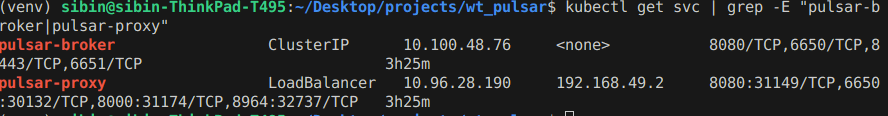
\includegraphics[width=0.8\textwidth]{implementation/pulsar-svcs.png}
    \caption{Pulsar Kubernetes Services}
    \label{fig:kgetpods}
\end{figure}

A sample Python consumer was developed to demonstrate real-time message consumption, subscribing to a specified topic with a shared subscription type and reporting end-to-end latency:

\begin{lstlisting}[breaklines=true,basicstyle=\small\ttfamily,frame=single]
consumer = client.subscribe(TOPIC_NAME, SUBSCRIPTION_NAME,
                            consumer_type=pulsar.ConsumerType.Shared)
msg = consumer.receive(timeout_millis=5000)
\end{lstlisting}

This consumer supports real-time consumption of video, audio, or chat streams and is extensible to other topics, validating integration with the Pulsar cluster.

\begin{figure}[h!]
    \centering
    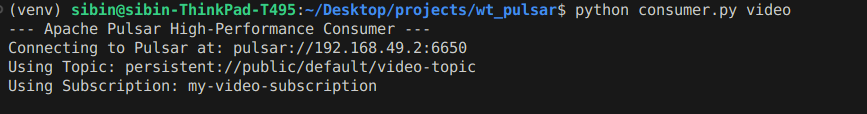
\includegraphics[width=0.8\textwidth]{implementation/consumer-video.png}
    \caption{Consumer Connection to Topic}
    \label{fig:consumer-conn}
\end{figure}

\begin{figure}[h!]
    \centering
    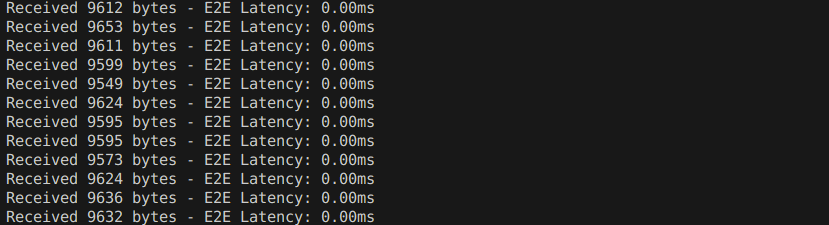
\includegraphics[width=0.8\textwidth]{implementation/pulsar-consumer-video.png}
    \caption{Consumer Receiving Data from Video Topic}
    \label{fig:consumer-data}
\end{figure}

% Describing retrieval of results
\subsection{Retrieving Results}
Metrics are logged in a CSV file within the router pod. To retrieve these files locally for evaluation, the following commands were executed:

\begin{lstlisting}[breaklines=true,basicstyle=\small\ttfamily,frame=single]
mkdir metrics-in-pod
kubectl cp webtransport-router-deployment-65cf75d584-njmqf:/app/metrics_logs ./metrics-in-pod
\end{lstlisting}

This process transfers the CSV files to the local machine, enabling detailed analysis of the system’s performance metrics.



% \section{Kubernetes Deployment}
% This implementation is the most important for the completion of our proposed solution. The router code is responsible to load balance streams of live data to seperate microservers. The router, microservice code and pulsar components are to be deployed into our kubernetes environment in minikube cluster

% \subsection{Deployment Secrets}
% To run our router in order to listen for Webtransport streams, there is a need for kubernetes to store our certficates. Certificates can be stored as secrets as detailed in Section 2.6.2, in the cluster. The generated certificate from Section 5.3 can be deployed into our kubernetes cluster so any entity in the namespace can access our certificate when mounted on a path.

% The following steps were done

% kubectl create secret tls quic-cert --cert=path/.crt --key=path/.key
% This creates a secret in kubernetes in the default namespace so all resources in the namespace can access it


% \subsection{Router Deployment}
% Router deployment was done with the steps  Containerization, creating configmaps, deployment, and service

% The router section in the implementation defines how the config file was constructed with hot reloading

% the router code was built with a docker file defined in --. This file was placed in the same directory as where the router code is and keeping the router\_config file outside. 

% docker build -t sbnm007/quic\_router:0.0.0 . 
% This built the docker image

% I pushed the docker image to dockerhub repository
% docker push sbnm007/quic\_router:0.0.0 

% Now we have successfully created a container image for our router which can be deployed to our cluster

% Firstly the router\_config file which we didnt create along with the iamge is deployed as a config map whihc allows for kubernetes managed configuration. This is a practice in k8s where parameters are put in config to allow for extensibility. In this case, the config file is used for addding or removing microservices by configuring the endpoints. This allows for change withing a single file without creating new image and avoids hard coding values. 

% The `mentioned in --router.yaml` file is a complete Kubernetes configuration that sets up the WebTransport Router, enabling it to dynamically route different types of real-time data (like video, audio, and chat) to their respective microservices. First, a `ConfigMap` is defined that contains the `router_config.yaml`—a dynamic routing configuration file that supports hot-reloading without needing to restart the router. This configuration includes routing rules for each service, such as endpoint, port, data format, and custom headers. The `Deployment` section specifies how the router is deployed inside Kubernetes, including the Docker image, ports for QUIC/HTTP3, and volume mounts for the config file and TLS certificates. It is configured to run a single replica but can be scaled up for high availability. TLS certificates are securely injected into the container using a Kubernetes `Secret`, enabling encrypted communication over QUIC. Environment variables are used by the router application to locate the mounted configuration and certificate files. Finally, the `Service` of type `LoadBalancer` exposes the router externally, allowing clients to connect via TCP or UDP on port 443. This setup ensures that the router is easily configurable, scalable, and ready for production use with secure and dynamic traffic routing capabilities.


% kubectl apply -f router.yaml
% This creates all the resources defined in the yaml
% you can check for the rources

% kubectl get pods
% kubectl get svc -> the service will receive an external ip address from the metallb



% \subsection{Microservice Deployment}

% The \texttt{microservice.yaml} file defines the complete Kubernetes configuration required to deploy the individual microservices—\textbf{video}, \textbf{audio}, and \textbf{chat}—in a scalable and dynamically configurable manner. At the core of this setup is a shared \texttt{ConfigMap} named \texttt{microservice-app-config}, which contains the \texttt{microservice\_config.yaml} file. This configuration file is mounted into each microservice container at runtime and enables hot-reloading of critical settings such as the Pulsar broker URL and toggles for enabling or disabling message forwarding to Pulsar.

% Each microservice is deployed via a dedicated \texttt{Deployment} resource, which runs a Python-based service with arguments specifying its type and listening port. The shared configuration is mounted at \texttt{/config}, and its path is provided to the container via an environment variable. This design ensures that all microservices operate independently while adhering to a consistent configuration standard.

% To facilitate internal communication within the Kubernetes cluster, each microservice is exposed via a corresponding \texttt{ClusterIP} \texttt{Service}—on port \textbf{4434} for video, \textbf{4435} for audio, and \textbf{4436} for chat. This allows the WebTransport Router and other system components to route data reliably using internal DNS.

% The architecture is modular by design: new microservices can be introduced with minimal effort by replicating and modifying the relevant deployment and service blocks.

% Two key parameters in the configuration used for Pulsar integration are:

% \begin{verbatim}
% pulsar_broker_url: "pulsar://10.100.48.76:6650"
% end_to_pulsar: true
% \end{verbatim}

% These values are included in the \texttt{ConfigMap} to facilitate debugging and operational control over Pulsar connectivity.


% \subsection{Pulsar Deployment}

% Deploying Apache Pulsar within a constrained local development environment, specifically using Minikube, posed significant challenges. The official Helm chart provided in the Apache Pulsar documentation proved unsuitable in this context, primarily due to repeated out-of-memory (OOM) issues encountered in the init containers, which were followed by failures in the BookKeeper nodes.

% To address these issues, an alternative Helm chart—maintained by DataStax and tailored for lightweight development environments—was used. This approach facilitated a successful deployment and also enabled exposure of the Pulsar broker outside the Kubernetes cluster. The following steps summarize the installation process:

% \begin{itemize}
%     \item Add the custom Helm chart repository:
%     \begin{verbatim}
%     helm repo add datastax-pulsar https://datastax.github.io/pulsar-helm-chart
%     \end{verbatim}

%     \item Update the Helm repository to fetch the latest charts:
%     \begin{verbatim}
%     helm repo update
%     \end{verbatim}

%     \item Download the example development configuration:
%     \begin{verbatim}
%     curl -LOs https://datastax.github.io/pulsar-helm-chart/examples/dev-values.yaml
%     \end{verbatim}

%     \item Modify \texttt{dev-values.yaml} to disable monitoring by setting:
%     \begin{verbatim}
%     kube-prometheus-stack:
%       enabled: false
%     \end{verbatim}
%     This change was essential to reduce resource consumption and ensure stability on limited hardware.

%     \item Deploy Pulsar with the modified configuration:
%     \begin{verbatim}
%     helm install pulsar -f dev-values.yaml datastax-pulsar/pulsar
%     \end{verbatim}
% \end{itemize}

% This deployment results in two essential services: \texttt{pulsar-broker}, which provides the internal message brokering functionality, and \texttt{pulsar-proxy}, which facilitates external access to the Pulsar ecosystem. 

% \begin{figure}[h!]
%     \centering
%     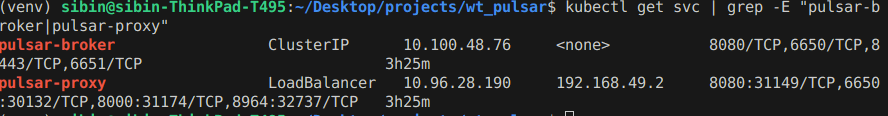
\includegraphics[width=0.8\textwidth]{implementation/pulsar-svcs.png}
%     \caption{Pulsar K8s Services}
%     \label{fig:kgetpods}
% \end{figure}



% For in-cluster applications—such as the microservices discussed earlier—communication with Pulsar occurs via the ClusterIP of the \texttt{pulsar-broker}. This enables efficient internal streaming to topics hosted within the Kubernetes network.

% For external consumers, connectivity is established via the \texttt{pulsar-proxy}, whose endpoint is exposed using a MetalLB load balancer. This approach ensures that consumers outside the Kubernetes cluster can access Pulsar using a stable IP address.

% A sample Python consumer was developed to demonstrate real-time message consumption. The consumer subscribes to a specified topic using a shared subscription type and reports end-to-end latency for each received message. The connection parameters, such as topic name and subscription identifier, are passed as command-line arguments.

% \begin{verbatim}
% consumer = client.subscribe(TOPIC_NAME, SUBSCRIPTION_NAME,
%                             consumer_type=pulsar.ConsumerType.Shared)
% msg = consumer.receive(timeout_millis=5000)
% \end{verbatim}

% This consumer architecture supports multiple use cases, including the real-time consumption of video, audio, or chat streams, and can be extended to other topics as required. It validates the successful integration between external clients and the Pulsar cluster deployed within Kubernetes.

% # image of consumption
% \begin{figure}[h!]
%     \centering
%     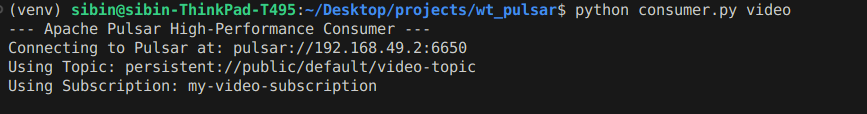
\includegraphics[width=0.8\textwidth]{implementation/consumer-video.png}
%     \caption{Consumer connection to topic}
%     \label{fig:consumer-conn}
% \end{figure}

% \begin{figure}[h!]
%     \centering
%     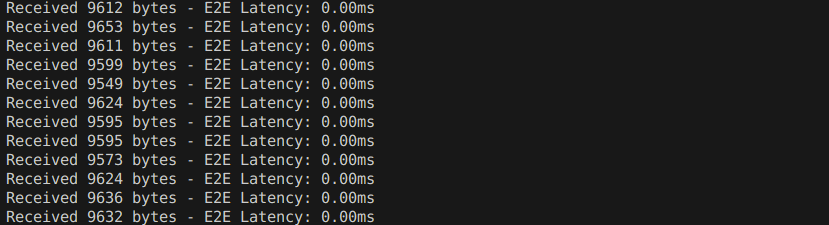
\includegraphics[width=0.8\textwidth]{implementation/pulsar-consumer-video.png}
%     \caption{Consumer Receiving Data from Video Topic}
%     \label{fig:consumer-data}
% \end{figure}




% \subsection{Getting the results}

% The CSV file is being logged inside the pod which captures our detailed metrics The following command is run to fetch the csv file to our local system
% mkdir metrics-in-pod
% kubectl cp webtransport-router-deployment-65cf75d584-njmqf:/app/metrics_logs ./metrics-in-pod
% With this we get the csv files in our local machien which we can evaluate

% \subsection{Pulsar Deployment}
% This part was particularly complex. I could not use the existing helm chart available in Apache Pulsar documentation. I faced issue where my init containers were giving OOM followed by bookie failure. I used alternative installation mechanism specifically for minikube by following the following steps

% Due to resource constaints I faced several challenges where my machine would go out of memory.
% I followed installation with this specific helm chart which made it work also helped to expose kafka broker out of kubernetes. 

% I ran the following commands
% This adds the custom chart  repo
% helm repo add datastax-pulsar https://datastax.github.io/pulsar-helm-chart

% helm repo update
% This gets the values.yaml file to my machine
% curl -LOs https://datastax.github.io/pulsar-helm-chart/examples/dev-values.yaml
% In this values.yaml I disable monitoring by setting kube-prometheus-stack: enabled : false so as to make my solution more efficient. 
% This applies the configuration and sets up our event broker service
% helm install pulsar -f dev-values.yaml datastax-pulsar/pulsar 

% This helm chart sets up pulsar-proxy as well as pulsar-broker 2 services which exposes end point for us to interact with apache pulsar. In this for our application code deployed in kuberentes we will use the cluster ip of the broker which allows us to push streams to respective topics within k8s


% For consumers sitting outside of pulsar, I will connect using pulsar-proxy endpoint which gets the ip address from my metal-lb load balancer.

% The consumer is a python code which connections to specified topic taken as command line arguments with new subscription. It also measures the end to end latency observed and successfully consumes the streams.

% % \\code
% % consumer = client.subscribe(TOPIC_NAME, SUBSCRIPTION_NAME, consumer_type=pulsar.ConsumerType.Shared)
% % msg = consumer.receive(timeout_millis=5000)


% Outside of my kubernetes cluster I consumers, this creates a subscription and connect to the respected pulsar topics and can consume respective streams in real-time. Following is the example of a consumer consuming from video topic

% 






% \section{Summary}

% The implementation began by setting up a local Kubernetes environment using Minikube with MetalLB for LoadBalancer functionality. TLS support was configured through self-signed certificates mapped to a custom domain, allowing secure WebTransport connections. A browser-based WebTransport client was built to stream multiple data types including video, audio, chat, files, and screen shares—each over distinct unidirectional QUIC streams. The client features a custom packet header format, real-time UI with live logs, and performance metrics. Wireshark was configured to decrypt QUIC traffic for validation using Chrome’s session keys.

% The WebTransport router, implemented in Python using aioquic, supports asynchronous QUIC + HTTP/3 stream handling, per-stream buffering, dynamic routing via a YAML config, and metrics logging. It forwards packets to generic microservices through a proxy layer. Each microservice processes packets based on type and can dynamically publish to Apache Pulsar using configurable producers and topic mapping. Pulsar was deployed with optimized Helm chart settings from DataStax to ensure stable operation in constrained local environments. Overall, the system successfully enables real-time multimedia streaming, processing, and message queuing—all managed within a fully containerized and configurable Kubernetes deployment.



\section{Network Traffic Analysis}
With both the WebTransport client and router implemented and deployed, this section demonstrates the actual network traffic captured during live streaming sessions. Using Wireshark with the previously configured TLS decryption, we can observe the real-time communication between the client and router, validating the implementation and providing insights into the protocol behavior.
\begin{figure}[h]
    \centering
    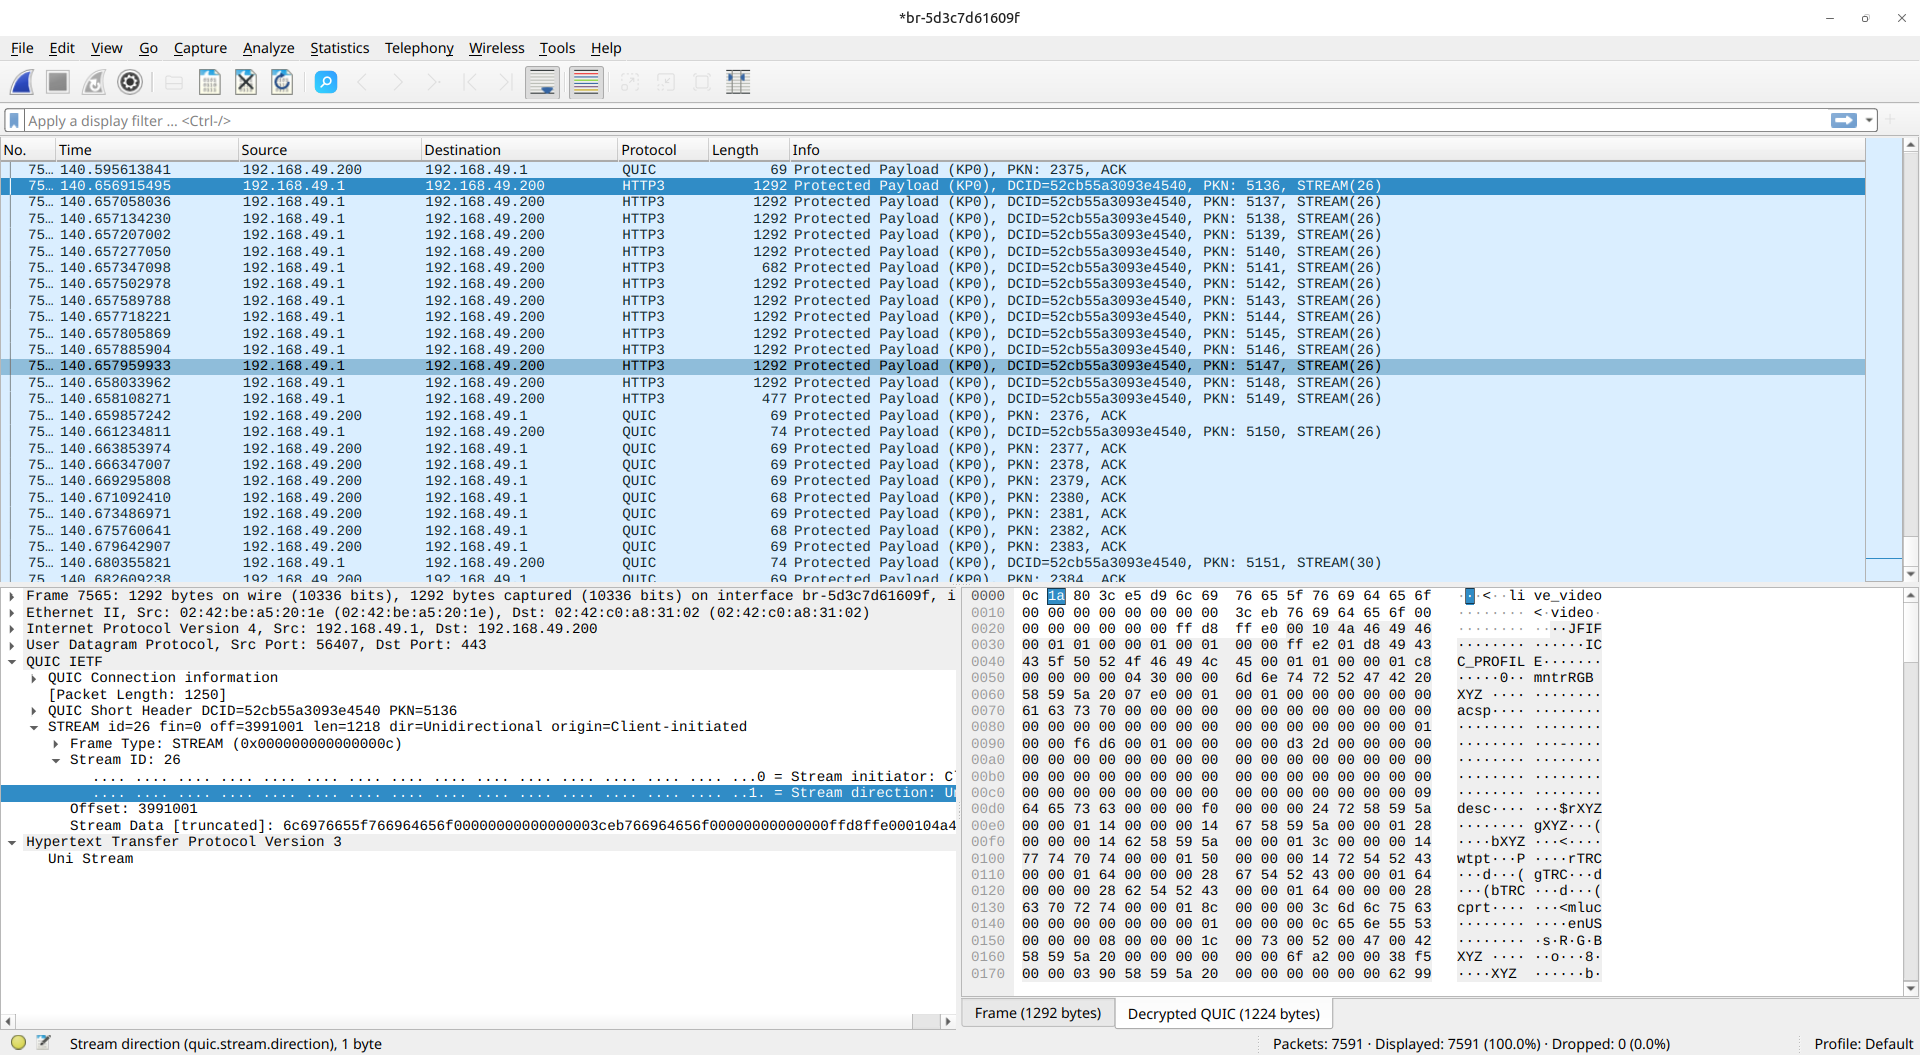
\includegraphics[width=0.8\textwidth]{implementation/network_traffic_analysis.png}
    \caption{Network Traffic Analysis using Wireshark}
    \label{fig:network_traffic_analysis}
\end{figure}


The figure \ref{fig:network_traffic_analysis} shows a snapshot of the network traffic captured on the 'br-5d3c7d61609f' network interface, which is where the custom router is deployed within the Kubernetes cluster. The source IP address 192.168.49.1 represents the WebTransport client, while the destination IP address 192.168.49.200 corresponds to the router's IP address exposed through MetalLB with a custom configured domain name.

The highlighted stream 26 demonstrates the HTTP/3 protocol implementation, with stream number 26 specifically handling live video data. Upon examining the decrypted QUIC packet in the bottom right panel, the packet structure begins with the expected 32-byte header containing the track identifier is correctly set to 'live\_video' as shown in the figure. The subsequent streams represent fragmented packets of the same stream type (live\_video), all maintaining the consistent stream ID 26, which validates the proper stream multiplexing implementation.

This captured traffic successfully validates the implementation of both the WebTransport client and router, demonstrating the successful transmission and processing of live video data. The network capture also reveals audio and chat packets transmitted over stream IDs 30 and 22 respectively, confirming the multi-stream architecture where different media types are isolated into separate streams to prevent head-of-line blocking.





\section{Summary}

In this chapter, a complete end-to-end prototype of the proposed system is implemented and validated within a local Kubernetes environment. The workflow begins with a browser-based WebTransport client that streams multiple types of media—such as video, audio, chat, and files—in real time using unidirectional QUIC streams. Each packet is formatted with a custom header and transmitted securely using TLS, with certificate handling and DNS mapping configured for seamless local development. The system demonstrates robust session management, live metrics collection, and a responsive user interface, enabling detailed insight into the streaming behavior.

The WebTransport router, deployed as a scalable microservice, acts as the central intelligence for traffic distribution. It uses asynchronous QUIC and HTTP/3 handling to buffer, parse, and dynamically route packets to the appropriate microservices based on a hot-reloadable YAML configuration. These backend microservices, implemented generically to support various media types, process the data and optionally publish it to Apache Pulsar topics for further stream processing or analytics. The deployment showcases critical infrastructure features such as TLS termination, local DNS resolution, zero-downtime scaling, and runtime observability—all orchestrated through Minikube, MetalLB, and Kubernetes-native tools. This working prototype not only verifies the architectural design but also lays a strong, extensible foundation for production-scale deployments or future research-driven enhancements.